\documentclass{article}
\usepackage{amsmath}
\usepackage{amsfonts}
\usepackage{amssymb}
\usepackage{amsthm}
\usepackage{xcolor}
\usepackage{geometry}[margin={1cm,1cm}]
\usepackage{graphicx}

\newtheorem{thm}{Theorem}
\newtheorem{lem}[thm]{Lemma}
\newtheorem{cor}[thm]{Corollary}
\newtheorem{defn}[thm]{Definition}

\author{Ben Shirley}

\begin{document}

\section*{Question 1}
\begin{enumerate}
    \item[1]
        \begin{figure}[!htb]
            \centering
            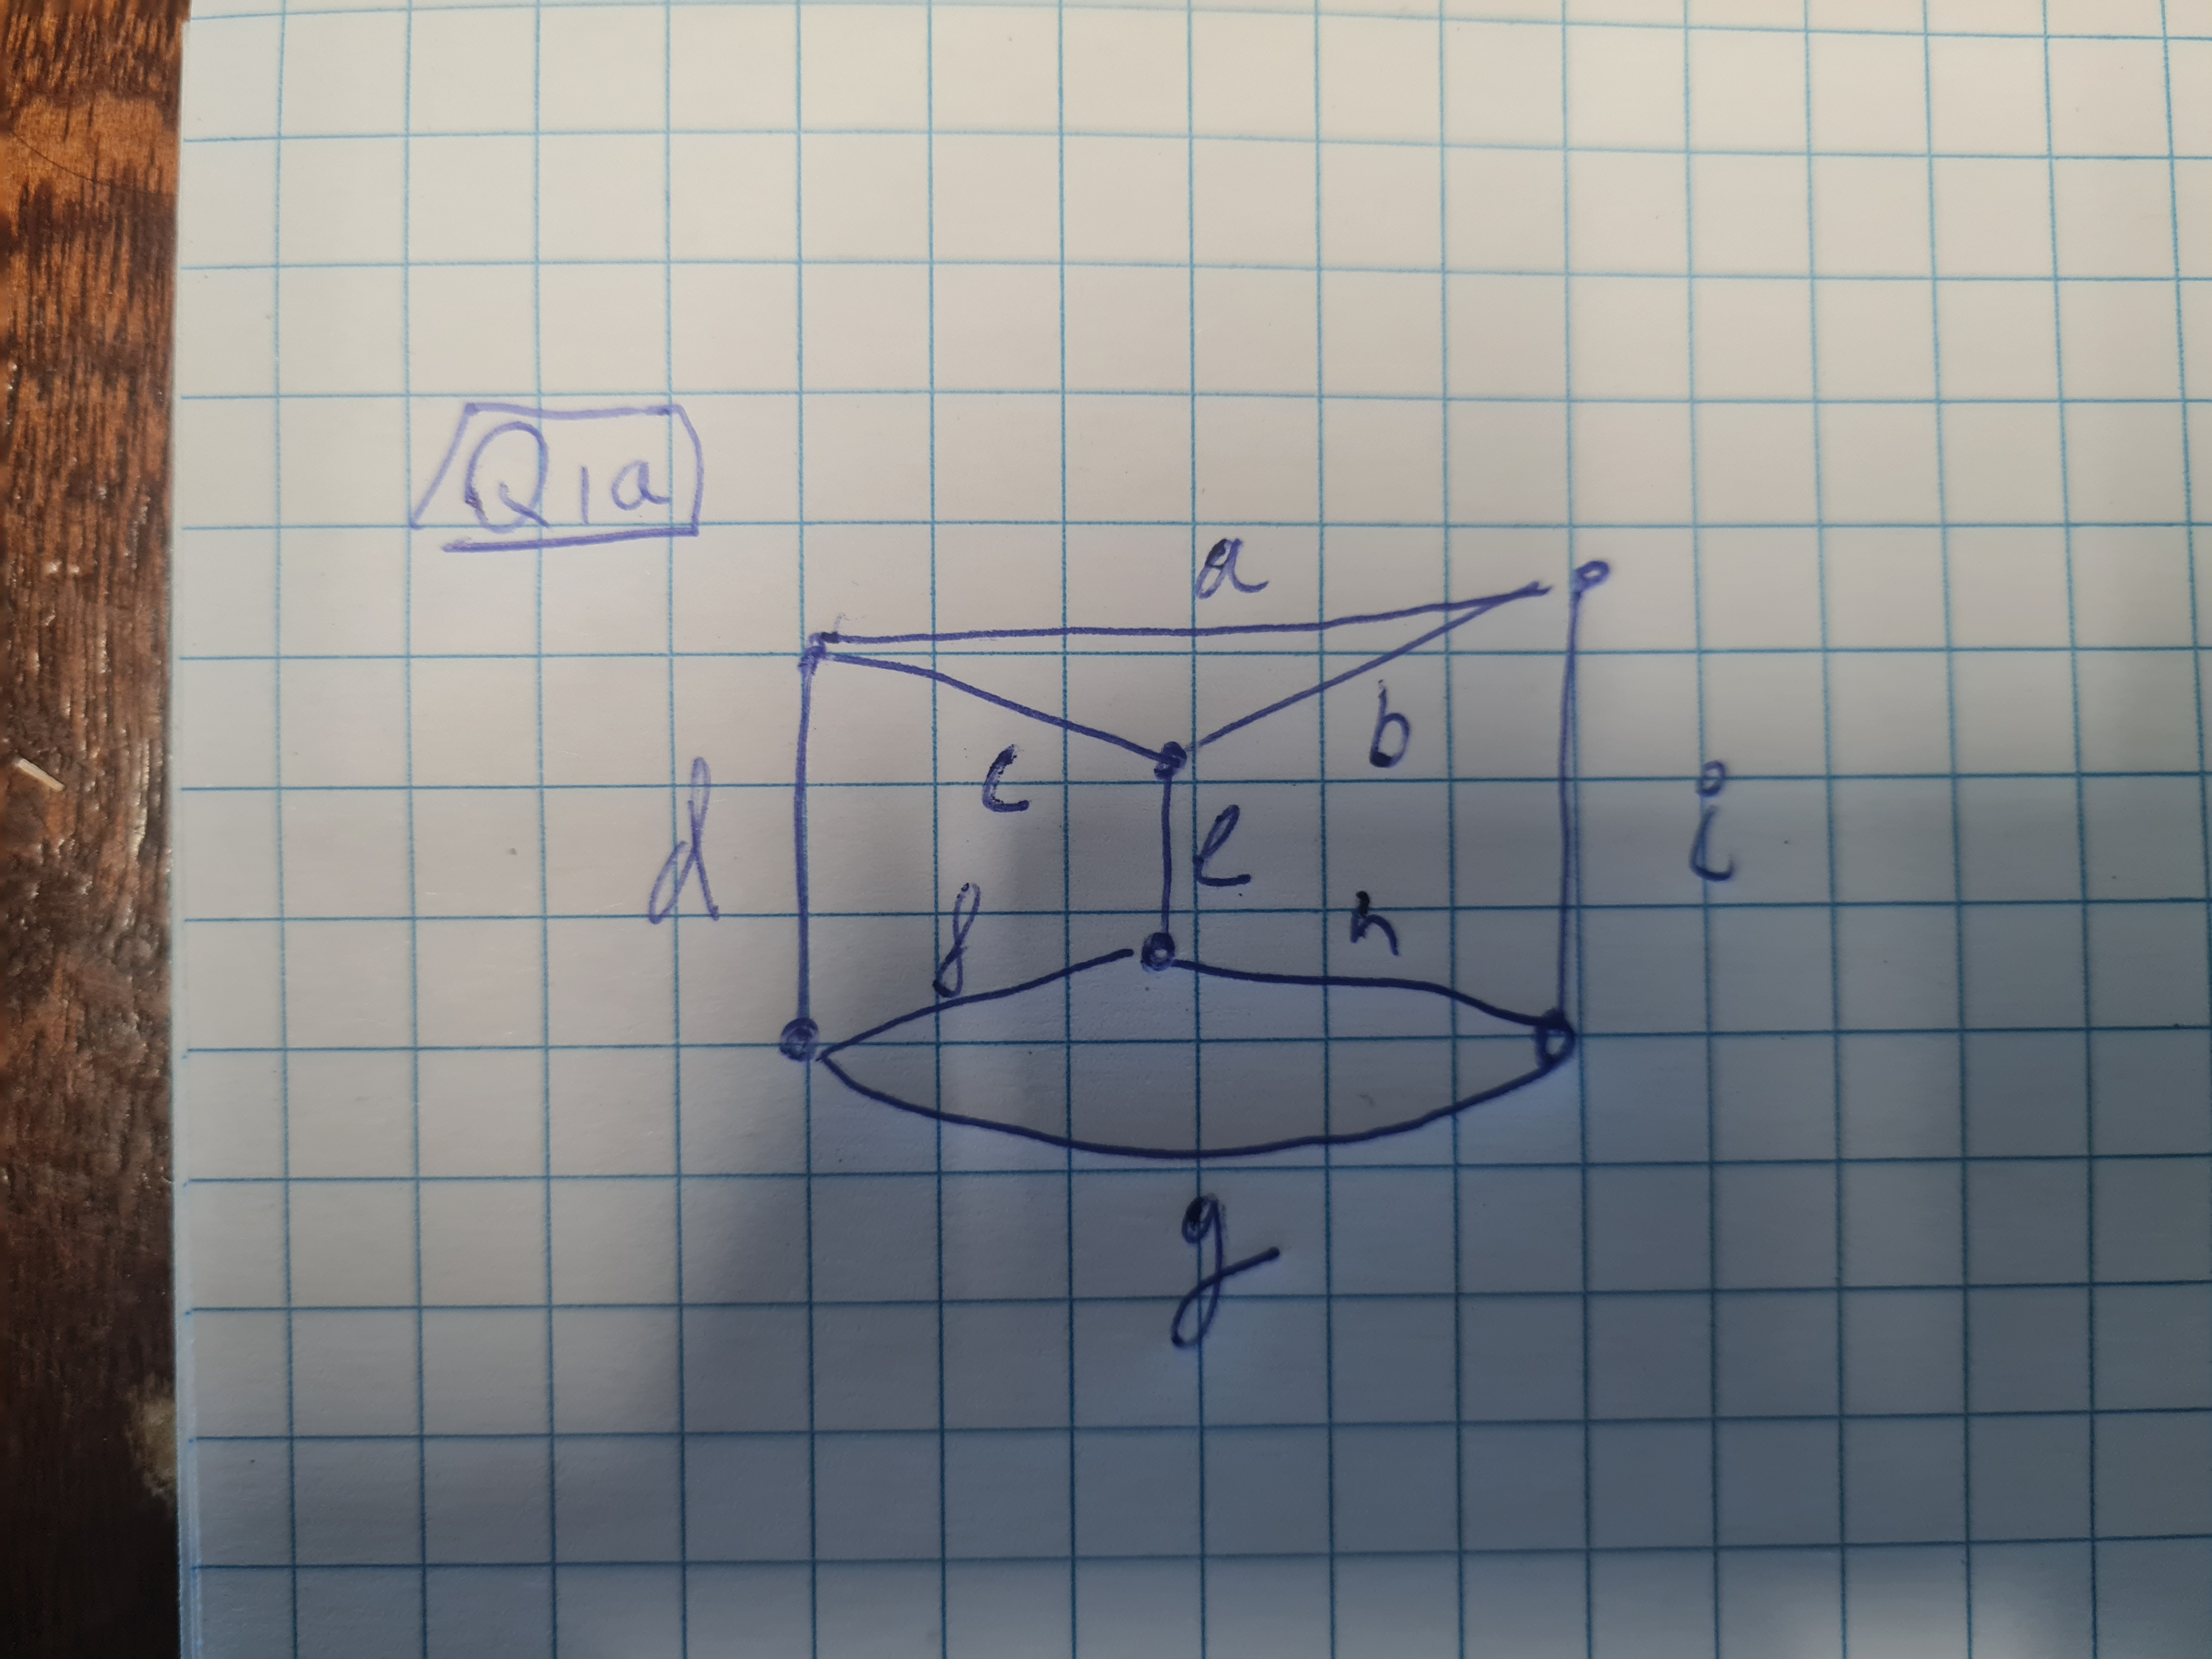
\includegraphics[width=0.5\textwidth]{q1a.jpg}
            \caption{Question 1 a}
        \end{figure}
    \item[2]
        \begin{figure}[!htb]
            \centering
            \includegraphics[width=0.5\textwidth]{q1b.jpg}
            \caption{Question 1 b}
        \end{figure}
    \item[3] As shown in class $M^*(G)=M(G^*)$,
        and so we draw a geometric representation of figure 2's 
        cycle matroid. Here a maximal tree has 4 verticies so 
        our bases are of size 4, so our geometric representation is in $\mathbb{R}^3$.

        First, notice that $\{f, h, b, c\}, \{f, h, d, i\}, \{d, i, b, c\}$ are all coplanar, and furthermore, we have $\{e, f, h\}, \{e, d, i\}$ 
        and $\{e, b, c\}$ all colinear. These elements must therefore form some sort of triangular pyramid.
        To see how $a, g$ fit into the picture, note that we have $\{a, g, c, f\}, \{a, g, b, h\}, \{f, c, b, h\}$ all coplanar.
        Furthermore, $\{d, f, g\}, \{d,c,a\}$ are colinear, as are $\{i, b, a\}, \{i, h, g\}$. So these elements do not form a pyramid,
        and instead form a weird 3d shape (plz see picture).
        Furthermore, we observe that $e, a$ and $e, g$ are involved in no common cycles of length $\le 4$. Putting this together we obtain the 
        following geometric representation.
        \begin{figure}
            \centering
            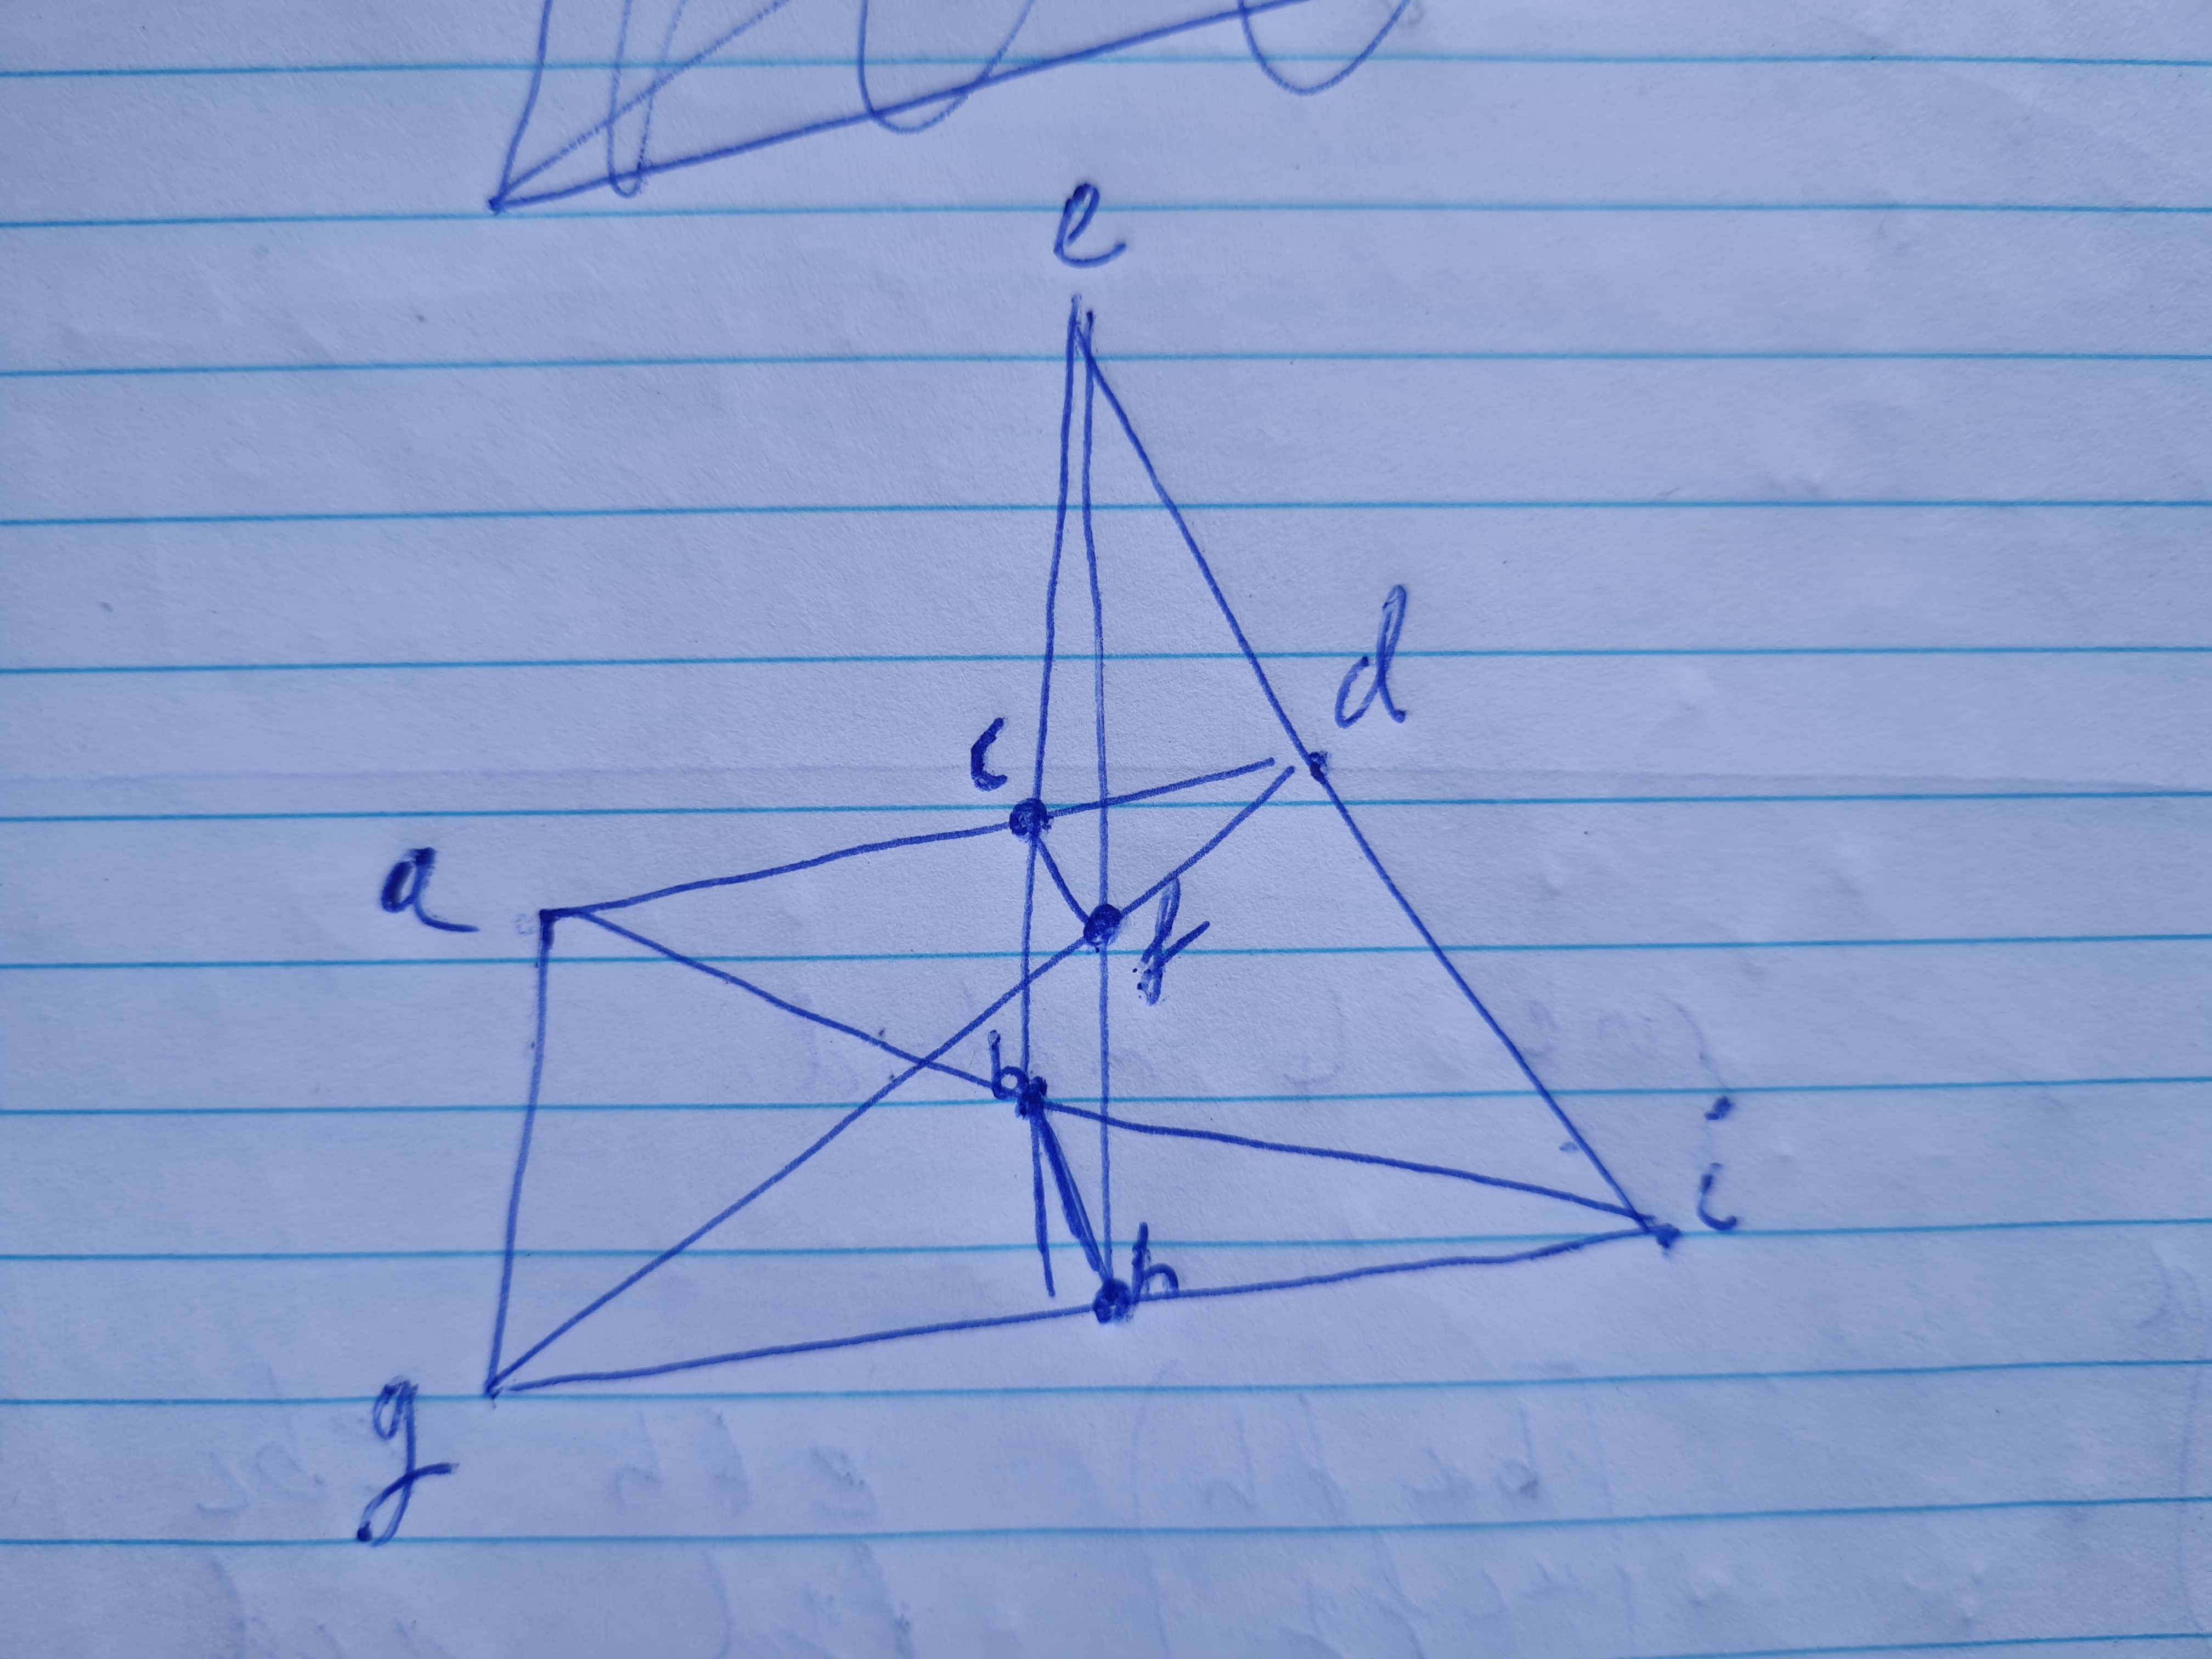
\includegraphics[width=0.5\textwidth]{q1c.jpg}
            \caption{Question 1 c}
        \end{figure}
        
\end{enumerate}

\section*{Question 2}
\begin{enumerate}
    \item[1] We perform the following operations: $R_2\to R_2+R_1$, $R_3\to R_3+4R_1$, $R_3\to R_3+4R_2$.
        $R_1\to R_1-R_3$, $R_2\to R_2-R_3$, $R_3\to 3R_3$.
        Following this we obtain the following matrix:
        \[
            \bordermatrix{
                & a & b & c & d & e & f & g \cr
                & 1 & 0 & 0 & 1 & 1 & 0 & 1 \cr
                & 0 & 1 & 0 & 1 & 0 & 1 & 3 \cr
                & 0 & 0 & 1 & 0 & 1 & 1 & 3 
            }
        \]
    \item[2] This is a rank 3 matroid, so we draw its geometric representation in the plane.
        Initially, we see that $a, b, c$ is independent, and so is $\{d, e, f\}$. Using the determinate 
        trick from class, it is easy to determine that $\{a, b, d\}, \{b, c, f\}, \{a, c, e\}$ are all dependent,
        as their corresponding matrices are the $1\times 1$, $[0]$ matrix. Similar checks will show that all other 3-element sets (not containing $g$)
        are independent. Finally, we see that $\{f, g, a\}$ is dependent, and all other matricies we might look at have zero determinate. 
        Hence, our geometric representation is:
        \begin{figure}[!htb]
            \centering
            \includegraphics[width=0.5\textwidth]{q2b.jpg}
            \caption{Question 2 b}
        \end{figure}


    \item[3] From class, we know that if $M=M([I|A])$, then $M^*=M([I|A^T])$. Now in reduced representation form, the rows are labeled by $\{a, b, c\}$,
        and columns by $\{d, e, f, g\}$. So, $A^T$ is labeled by $\{a, b, c\}$, and the identity matrix by $\{d, e, f, g\}$.
        \[
            \bordermatrix{
                & d & e & f & g & a & b & c \cr
                & 1 & 0 & 0 & 0 & 1 & 1 & 0 \cr
                & 0 & 1 & 0 & 0 & 1 & 0 & 1 \cr
                & 0 & 0 & 1 & 0 & 0 & 1 & 1 \cr
                & 0 & 0 & 0 & 1 & 1 & 3 & 3 
            }
        \]
    \item[3] Our geometric representation will be in $\mathbb{R}^3$, and we immediately see that $d, e, f, g$ are independent.
        Clearly, $\{a, d, e, g\}$ are coplanar, as are $\{b, d, f, g\}$ and $\{c, e, f, g\}$. In fact, removing any element from these sets 
        gives us an independent set, so these are in fact circuits.
        However, $\{a, b, c, g\}$ is independent, as viewing it in reduced representation, we see that 
        the determinate of the first 3 rows of $a, b, c$ is non-zero. Therefore, these are the only circuits \textbf{CHECK!}, 
        and our geometric representation is as follows:
        \begin{figure}
            \centering
            \caption{}
        \end{figure}
        
\end{enumerate}

\section*{Question 3}
Let $M$ be a matroid on ground set $E$ with independent sets $\mathcal{I}$, and $e\in E$ not be a loop in $M$.
Consider the set $A=\{I\subseteq E-e:I\cup e\in \mathcal{I}\}$. We will show that $A$ satisfies the independent set axioms.

\begin{enumerate}
    \item[I1] Firstly, note that $e$ is not a loop, and so $e\in\mathcal{I}$. Then $\emptyset$ has $\emptyset\cup e=\{e\}\in\mathcal{I}$
    and so $\emptyset\in A$.
    \item[I2] Now, suppose that $X\in A$ and $Y\subseteq X$. Then $Y\cup e\subseteq X\cup e\in\mathcal{I}$, and since $\mathcal{I}$
        is a family of independent sets, $Y\cup e\in\mathcal{I}$ too. Hence $Y\in A$.
    \item[I3] Suppose $X, Y\in A$ with $|X|<|Y|$. Then $X\cup e, Y\cup e\in\mathcal{I}$ with $|X\cup e|<|Y\cup e|$.
        So by applying I3 to $\mathcal{I}$, we can find some $a\in (Y\cup e)-(X\cup e)$ such that $X\cup e\cup a\in\mathcal{I}$.
        However, note that $a\ne e$, and clearly $a\not\in X$. So, we must have $a\in Y-X$ and thus $X\cup a\cup e\in\mathcal{I}$
        implies that $X\cup a\in A$ as required.

    Hence $A$ satisfies all required properties, showing $M/e$ is a matroid.
\end{enumerate}

\section*{Question 4}
\begin{enumerate}
    \item[a] We expect $r(M/a)=r(M)-1$, so our geometric representation will be in $\mathbb{R}^2$. Now $\{f, e, h, g, i\}$ is a hyperplane,
        and so we project onto this plane.
        \begin{figure}[!htb]
            \centering
            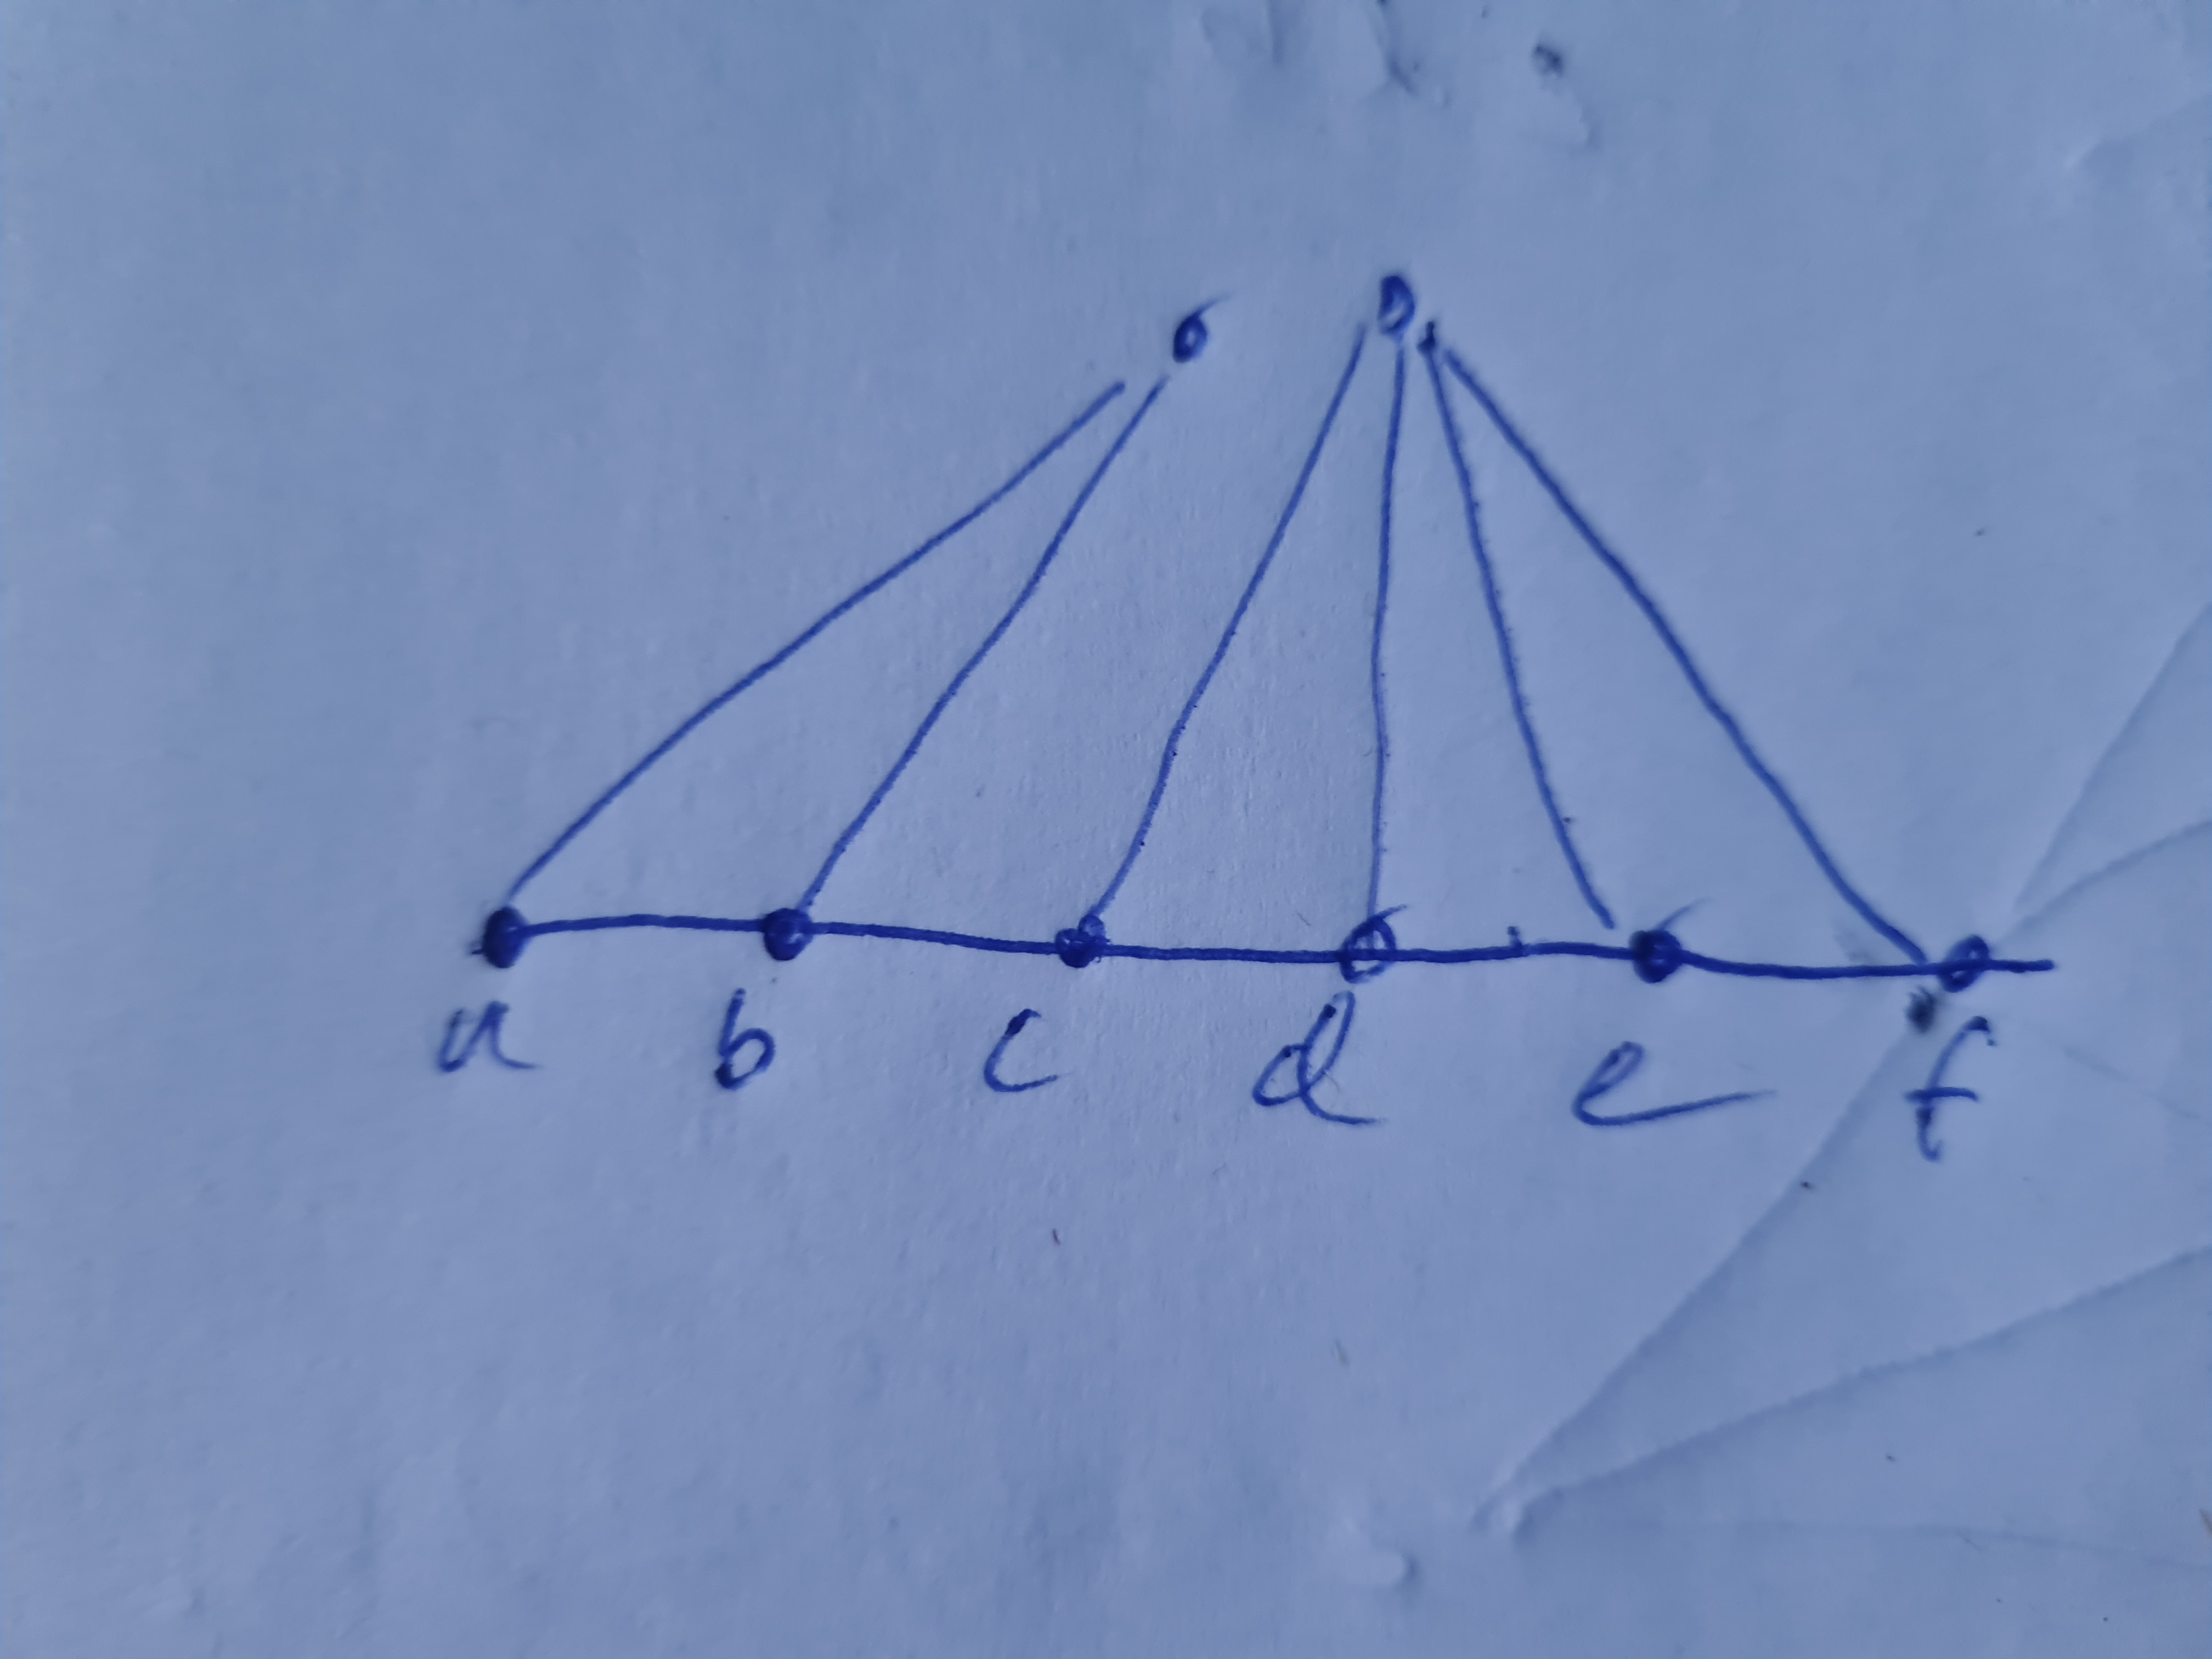
\includegraphics[width=0.5\textwidth, angle=-90]{q4a.jpg}
            \caption{Question 4 A}
        \end{figure}
    \item[b] Again, we use $\{f, e, h, g, i\}$ as our hyperplane
        \begin{figure}[!htb]
            \centering
            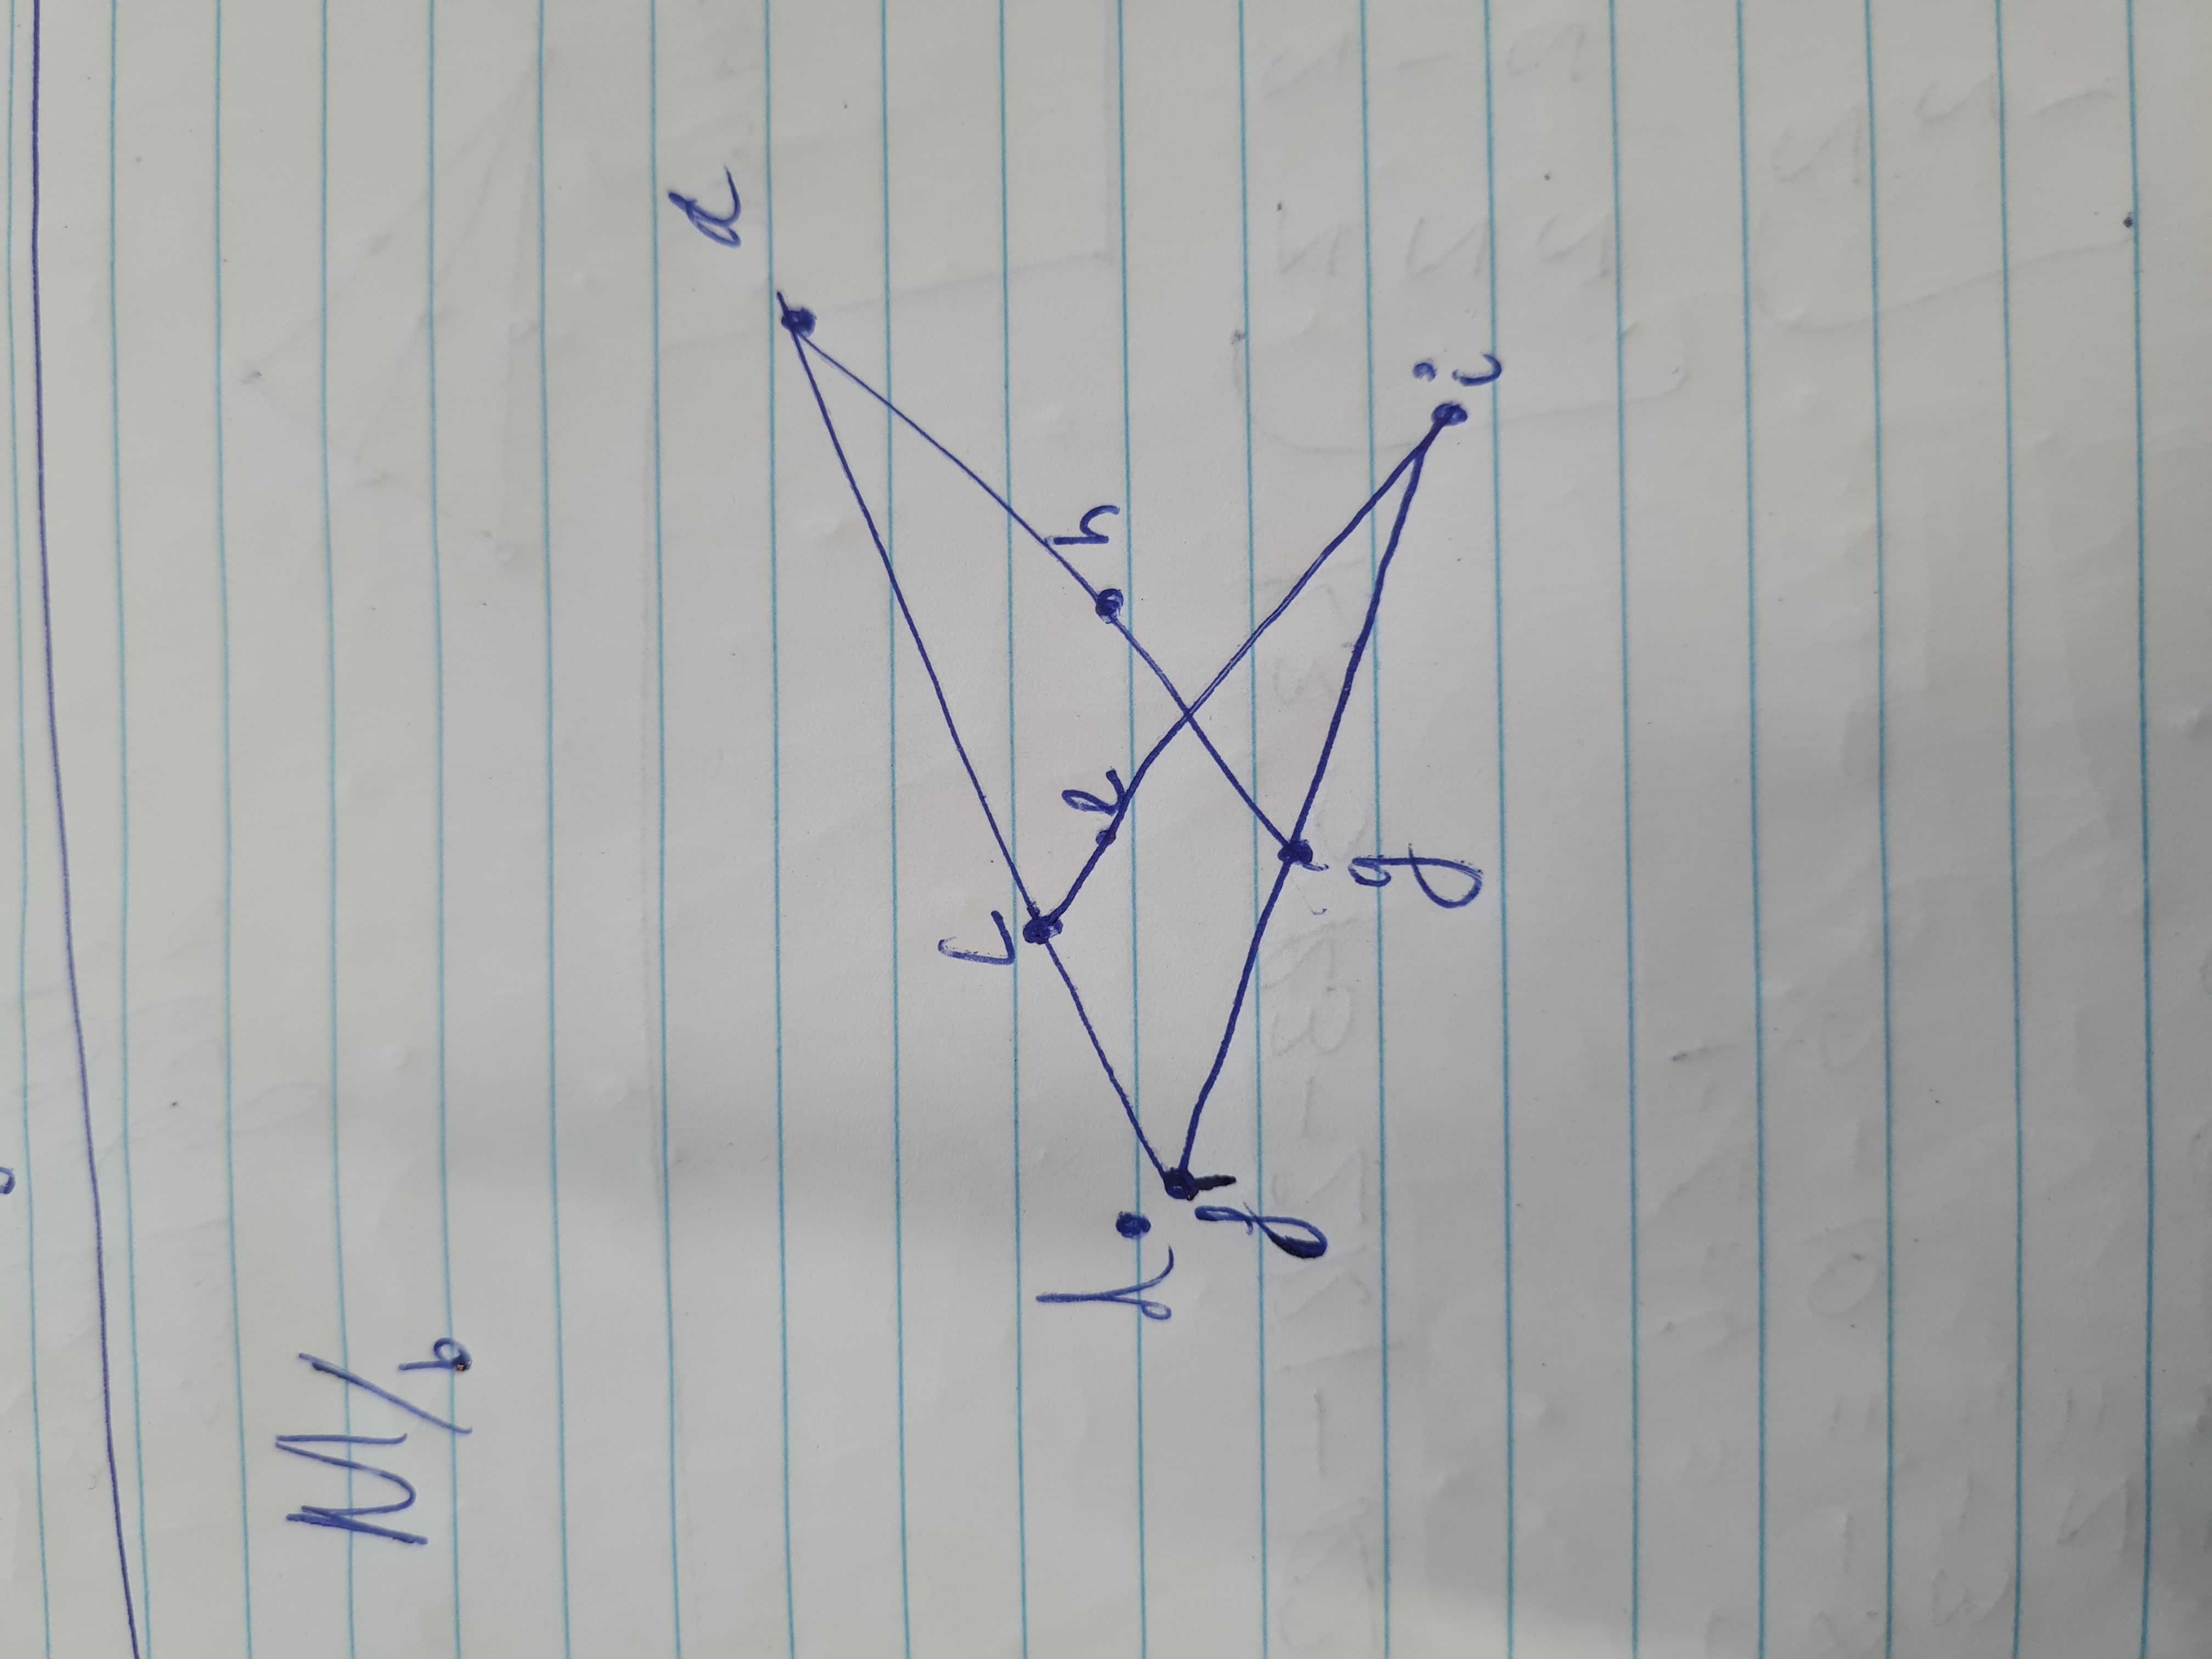
\includegraphics[width=0.5\textwidth, angle=-90]{q4b.jpg}
            \caption{Question 4 B}
        \end{figure}
    \item[c] We start with the geometric representation of $M/b$, and then delete $c, e$ and any redundant edges.
        In particular, the lines $\{d, f, a, c\}$ and $\{i, e, c\}$ become redundant.
        \begin{figure}
            \centering
            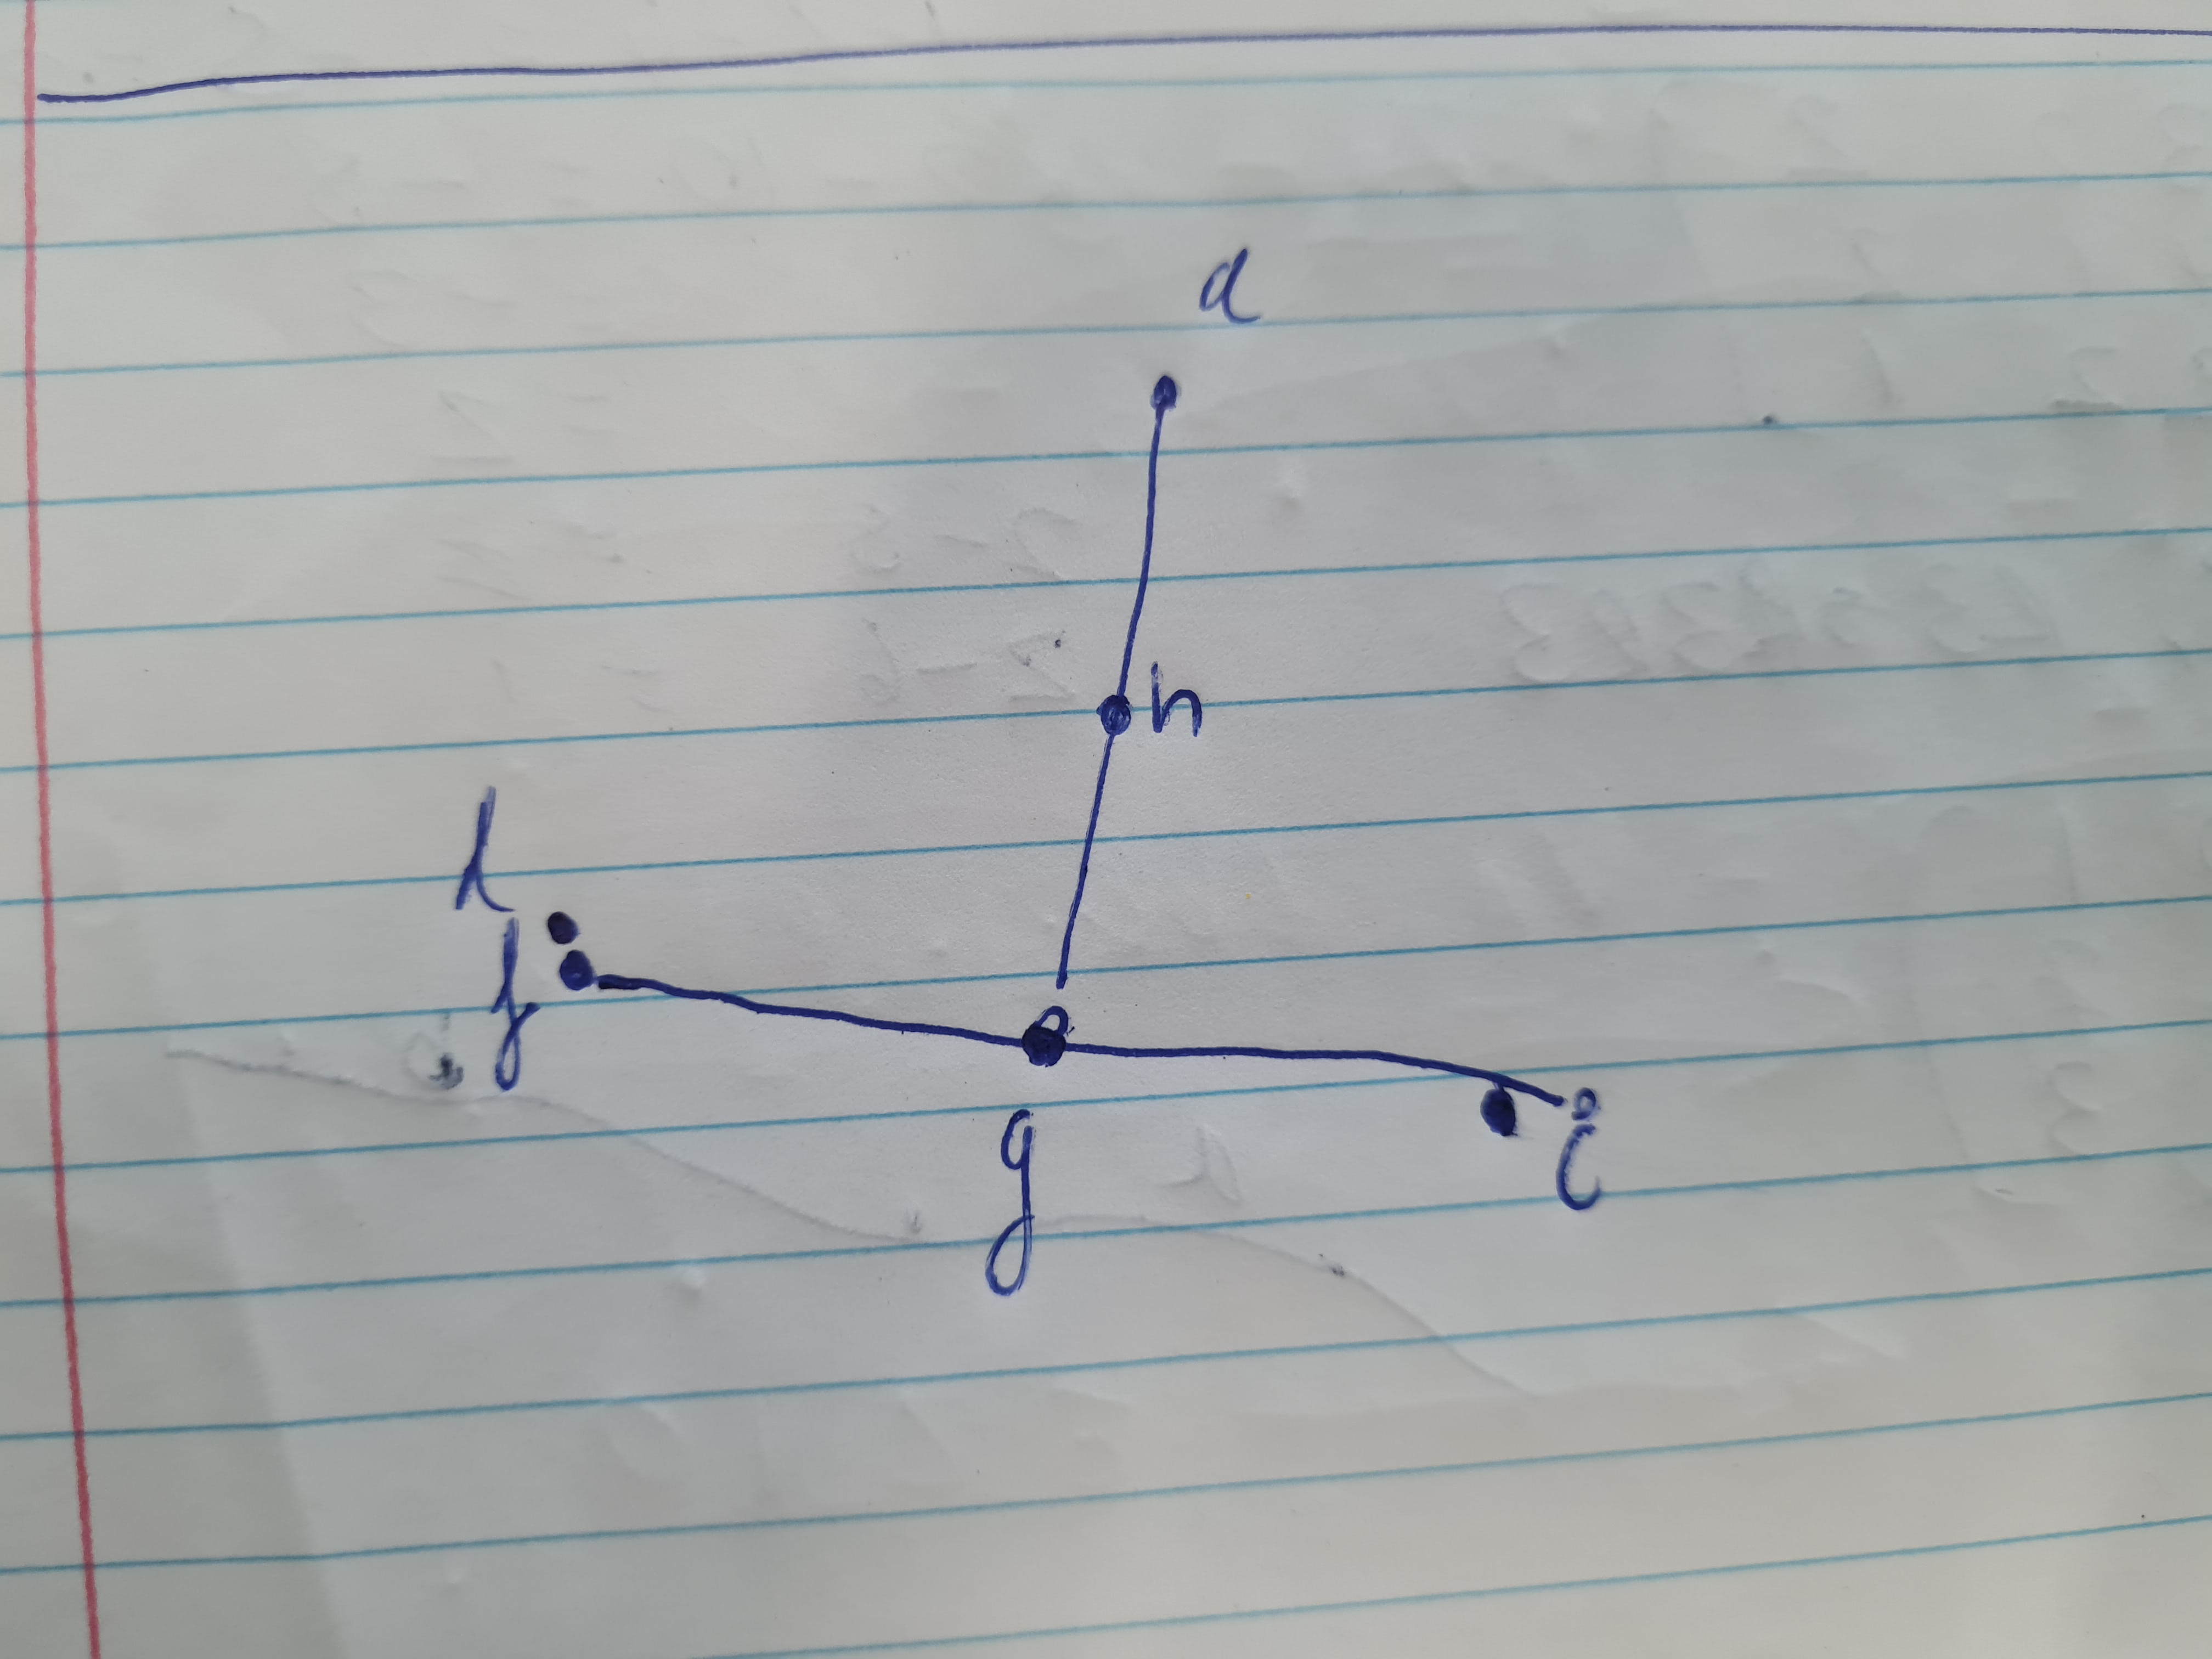
\includegraphics[width=0.5\textwidth]{q4c.jpg}
            \caption{Question 4 C}
        \end{figure}
    \item[d] For a contraction on $f$, we choose $\{g, e, c, a\}$ as our hyperplane.
        \begin{figure}
            \centering
            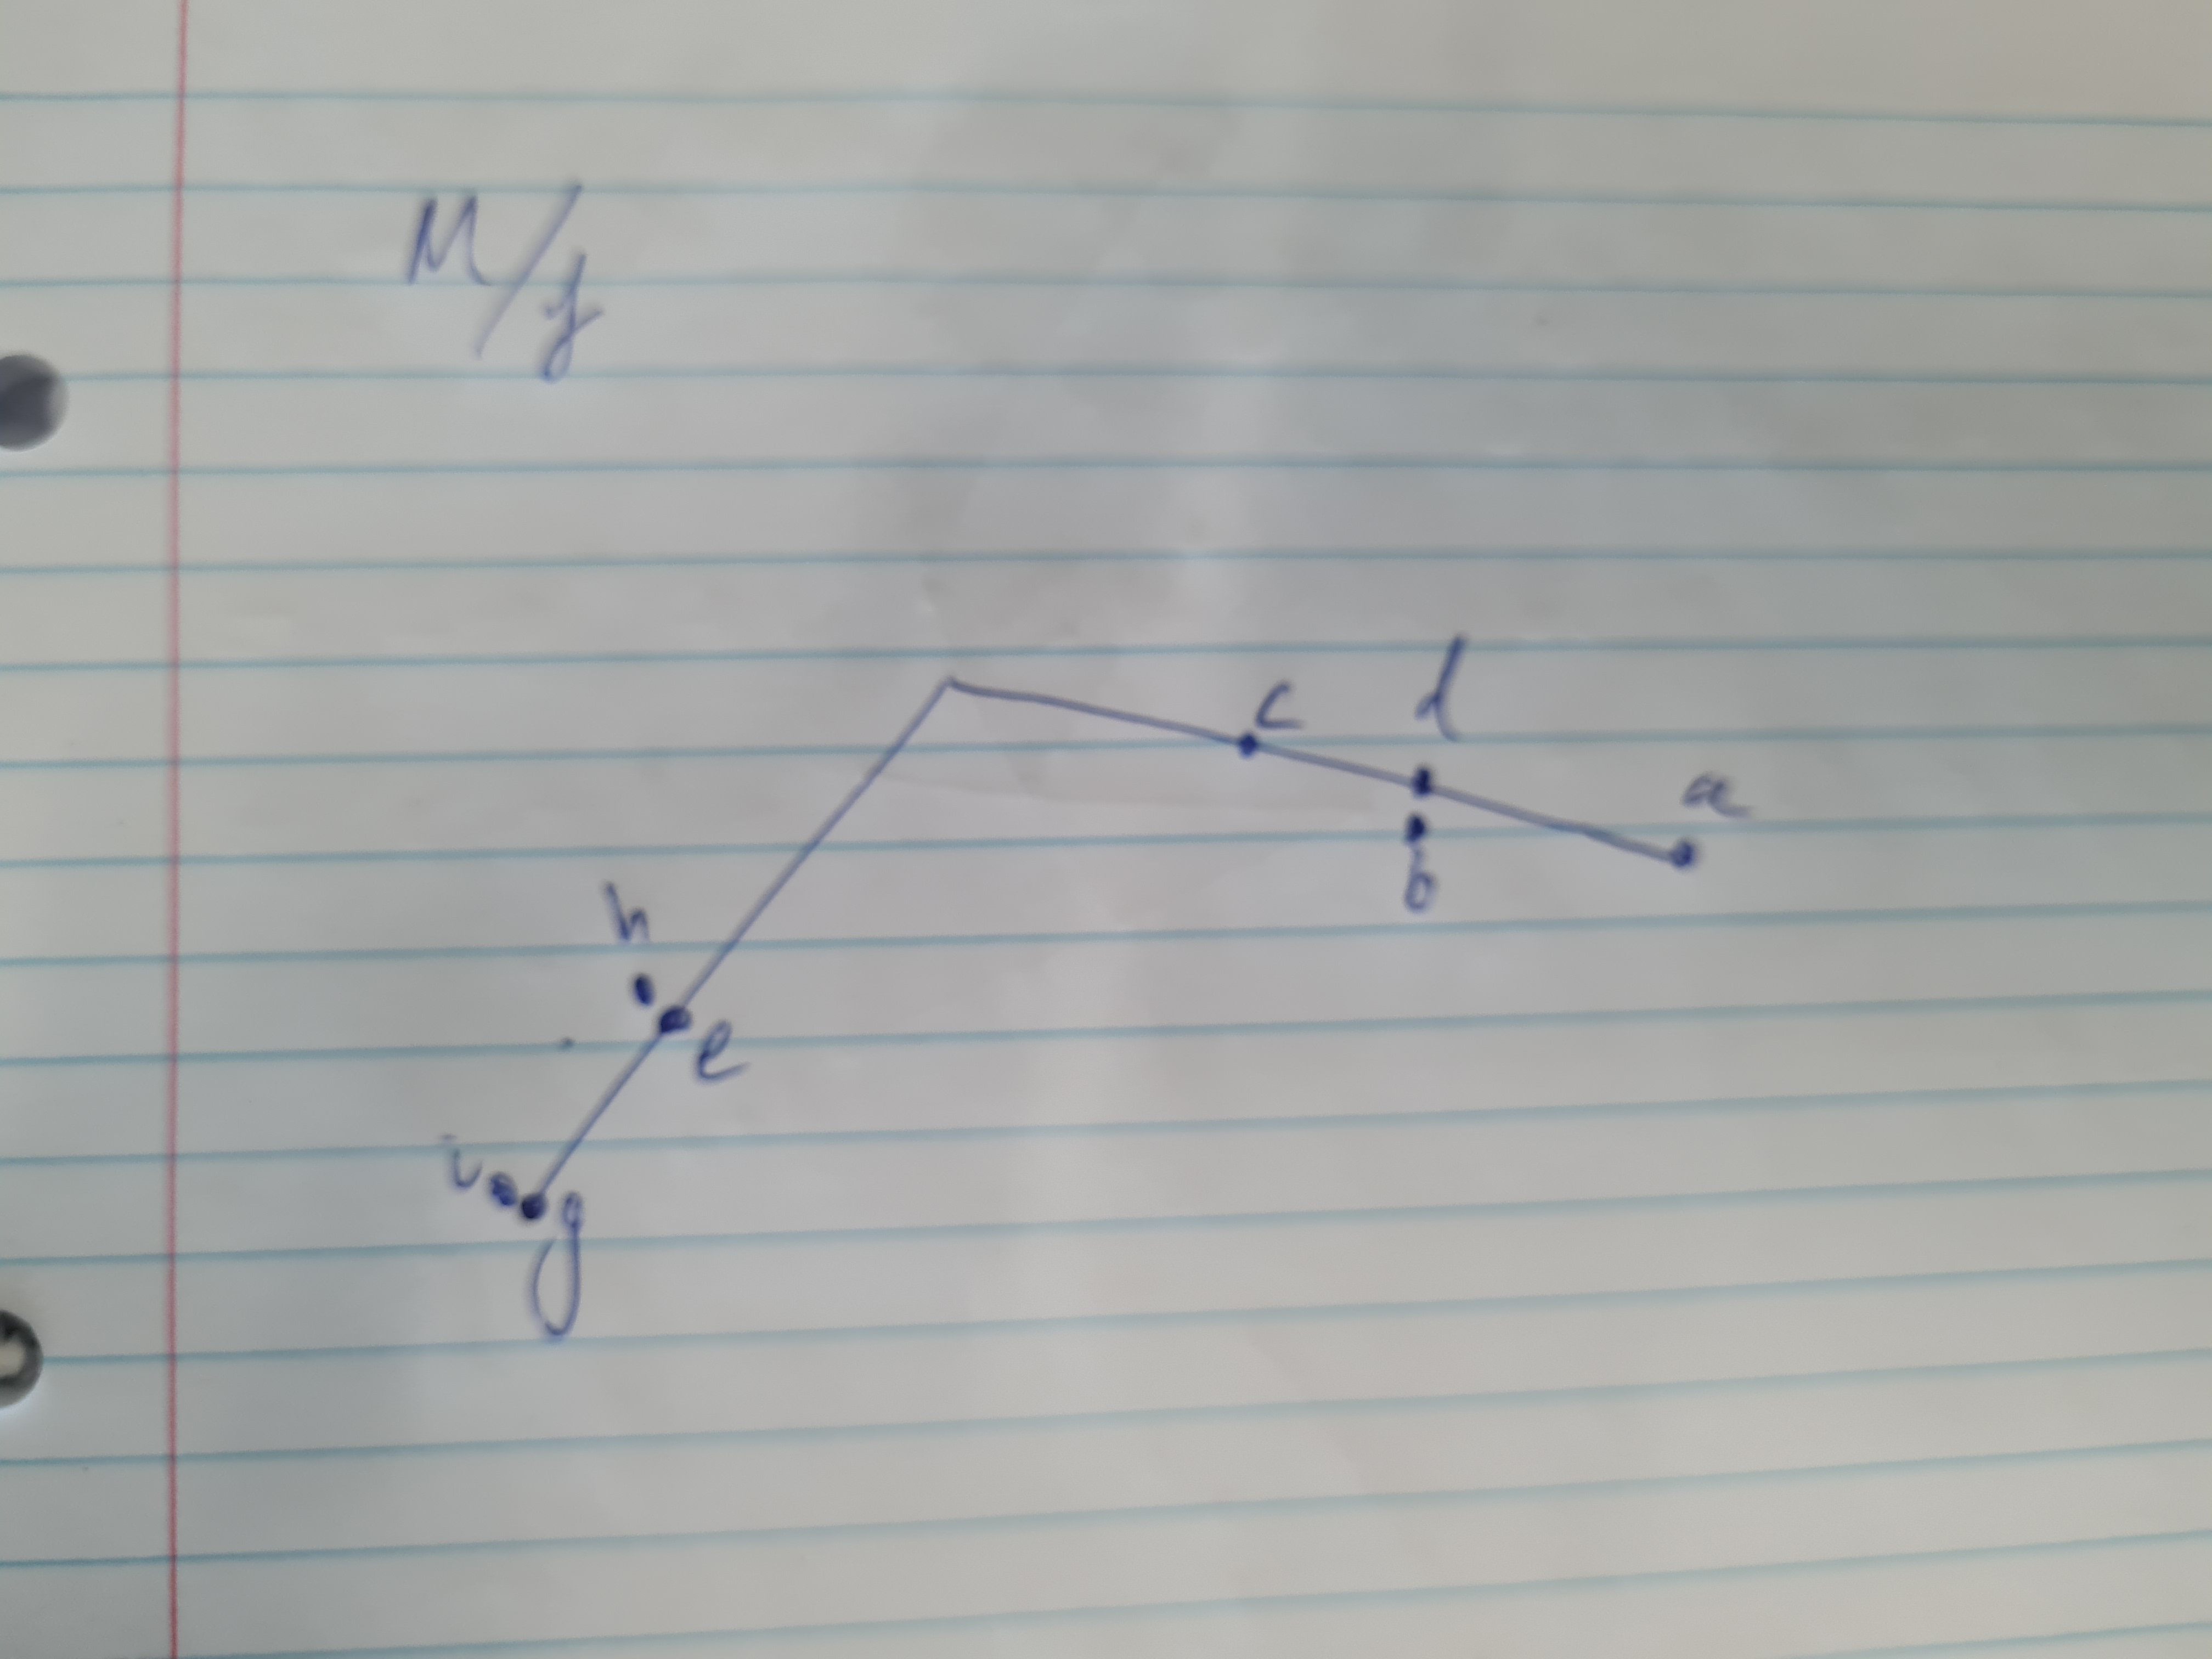
\includegraphics[width=0.5\textwidth]{q4d.jpg}
            \caption{Question 4 D}
        \end{figure}


\end{enumerate}
\section*{Question 5}
It suffices to show that for a sparse paving matroid, $M$, and $e\in E(M)$, that $M/e$ and $M\backslash e$ are sparse paving.
But in fact, we showed that sparse paving matroids are closed under duality, and in class we saw that $M/e=(M^*\backslash e)^*$,
so actually all we need to do is show that $M\backslash e$ is sparse paving.

Suppose first that $e$ is not a loop.
Now the independent sets of $M\backslash e$ are $\{C\in\mathcal{C}(M): e\not\in C\}$.
Now $r(M\backslash e)=r(M)=r$, so if $C, C'$ are circuits of size $r$ in $M\backslash e$, then they are circuits of size $r$ in $M$.
Hence by assumption $|C\cap C'|<r-1$. Thus $M\backslash e$ is sparse paving in this case.

In the second case, when $e$ is a loop, we have that $\{e\}$ is a circuit. Then the circuits of $M\backslash e$ are simply all circuits 
except this one. So again, the exact same reasoning will show that $M\backslash e$ is sparse paving

\textbf{TODO: more detail?}

\section*{Question 6}
\begin{enumerate}
    \item[$i\implies ii$] Suppose that $e\in E(M)$ is a coloop, and further that for some $X\subseteq E(M)$ that $e\in cl(X)$.
        Then $r(X\cup e)=r(X)$.

        Let $B_X\subseteq X$ be a maximal independent set contained in $X$. $B_X$ must extend to a basis, $B$ (it is an independent set),
        and since $e$ is a coloop, it must be in that basis. S
        o, if $e\not\in B_x$, then $B_X\cup e$ is independent, 
        and so $r(X)+1=r(B_X\cup e)\le r(X\cup e)=r(X)$, a contraction.

    \item[$ii\implies iii$] Suppose that for every $X\subseteq E(M)$ with $e\in cl(X)$, that $e\in X$.
        Now consider $X=E(M)-e$. $e\not\in X$, and so by assumption, $e\not\in cl(X)$
        But now, $X\subseteq cl(X)\subseteq E(M)-e=X$, and so $X$ is a flat. It remains to consider the rank of 
        $X$. We have $r(M)=r(X\cup e)\ne r(X)$ by assumption. Therefore as shown in class, we must have $r(X\cup e)=r(X)+1$,
        and so $r(X)=r(M)-1$, showing that $X$ is a hyperplane.

    \item[$iii\implies i$] If $E(M)-e$ is a hyperplane, then by definition $e$ is a coloop.\textbf{IS THIS CORRECT?}
\end{enumerate}

\section*{Question 6}
As seen in class, the Fano matroid serves as a valid example here. 
However, It is slightly easier to consider the matriod, $M$ (see figure), which is evidently transversal
as seen in the next figure.


\begin{figure}
    \centering
            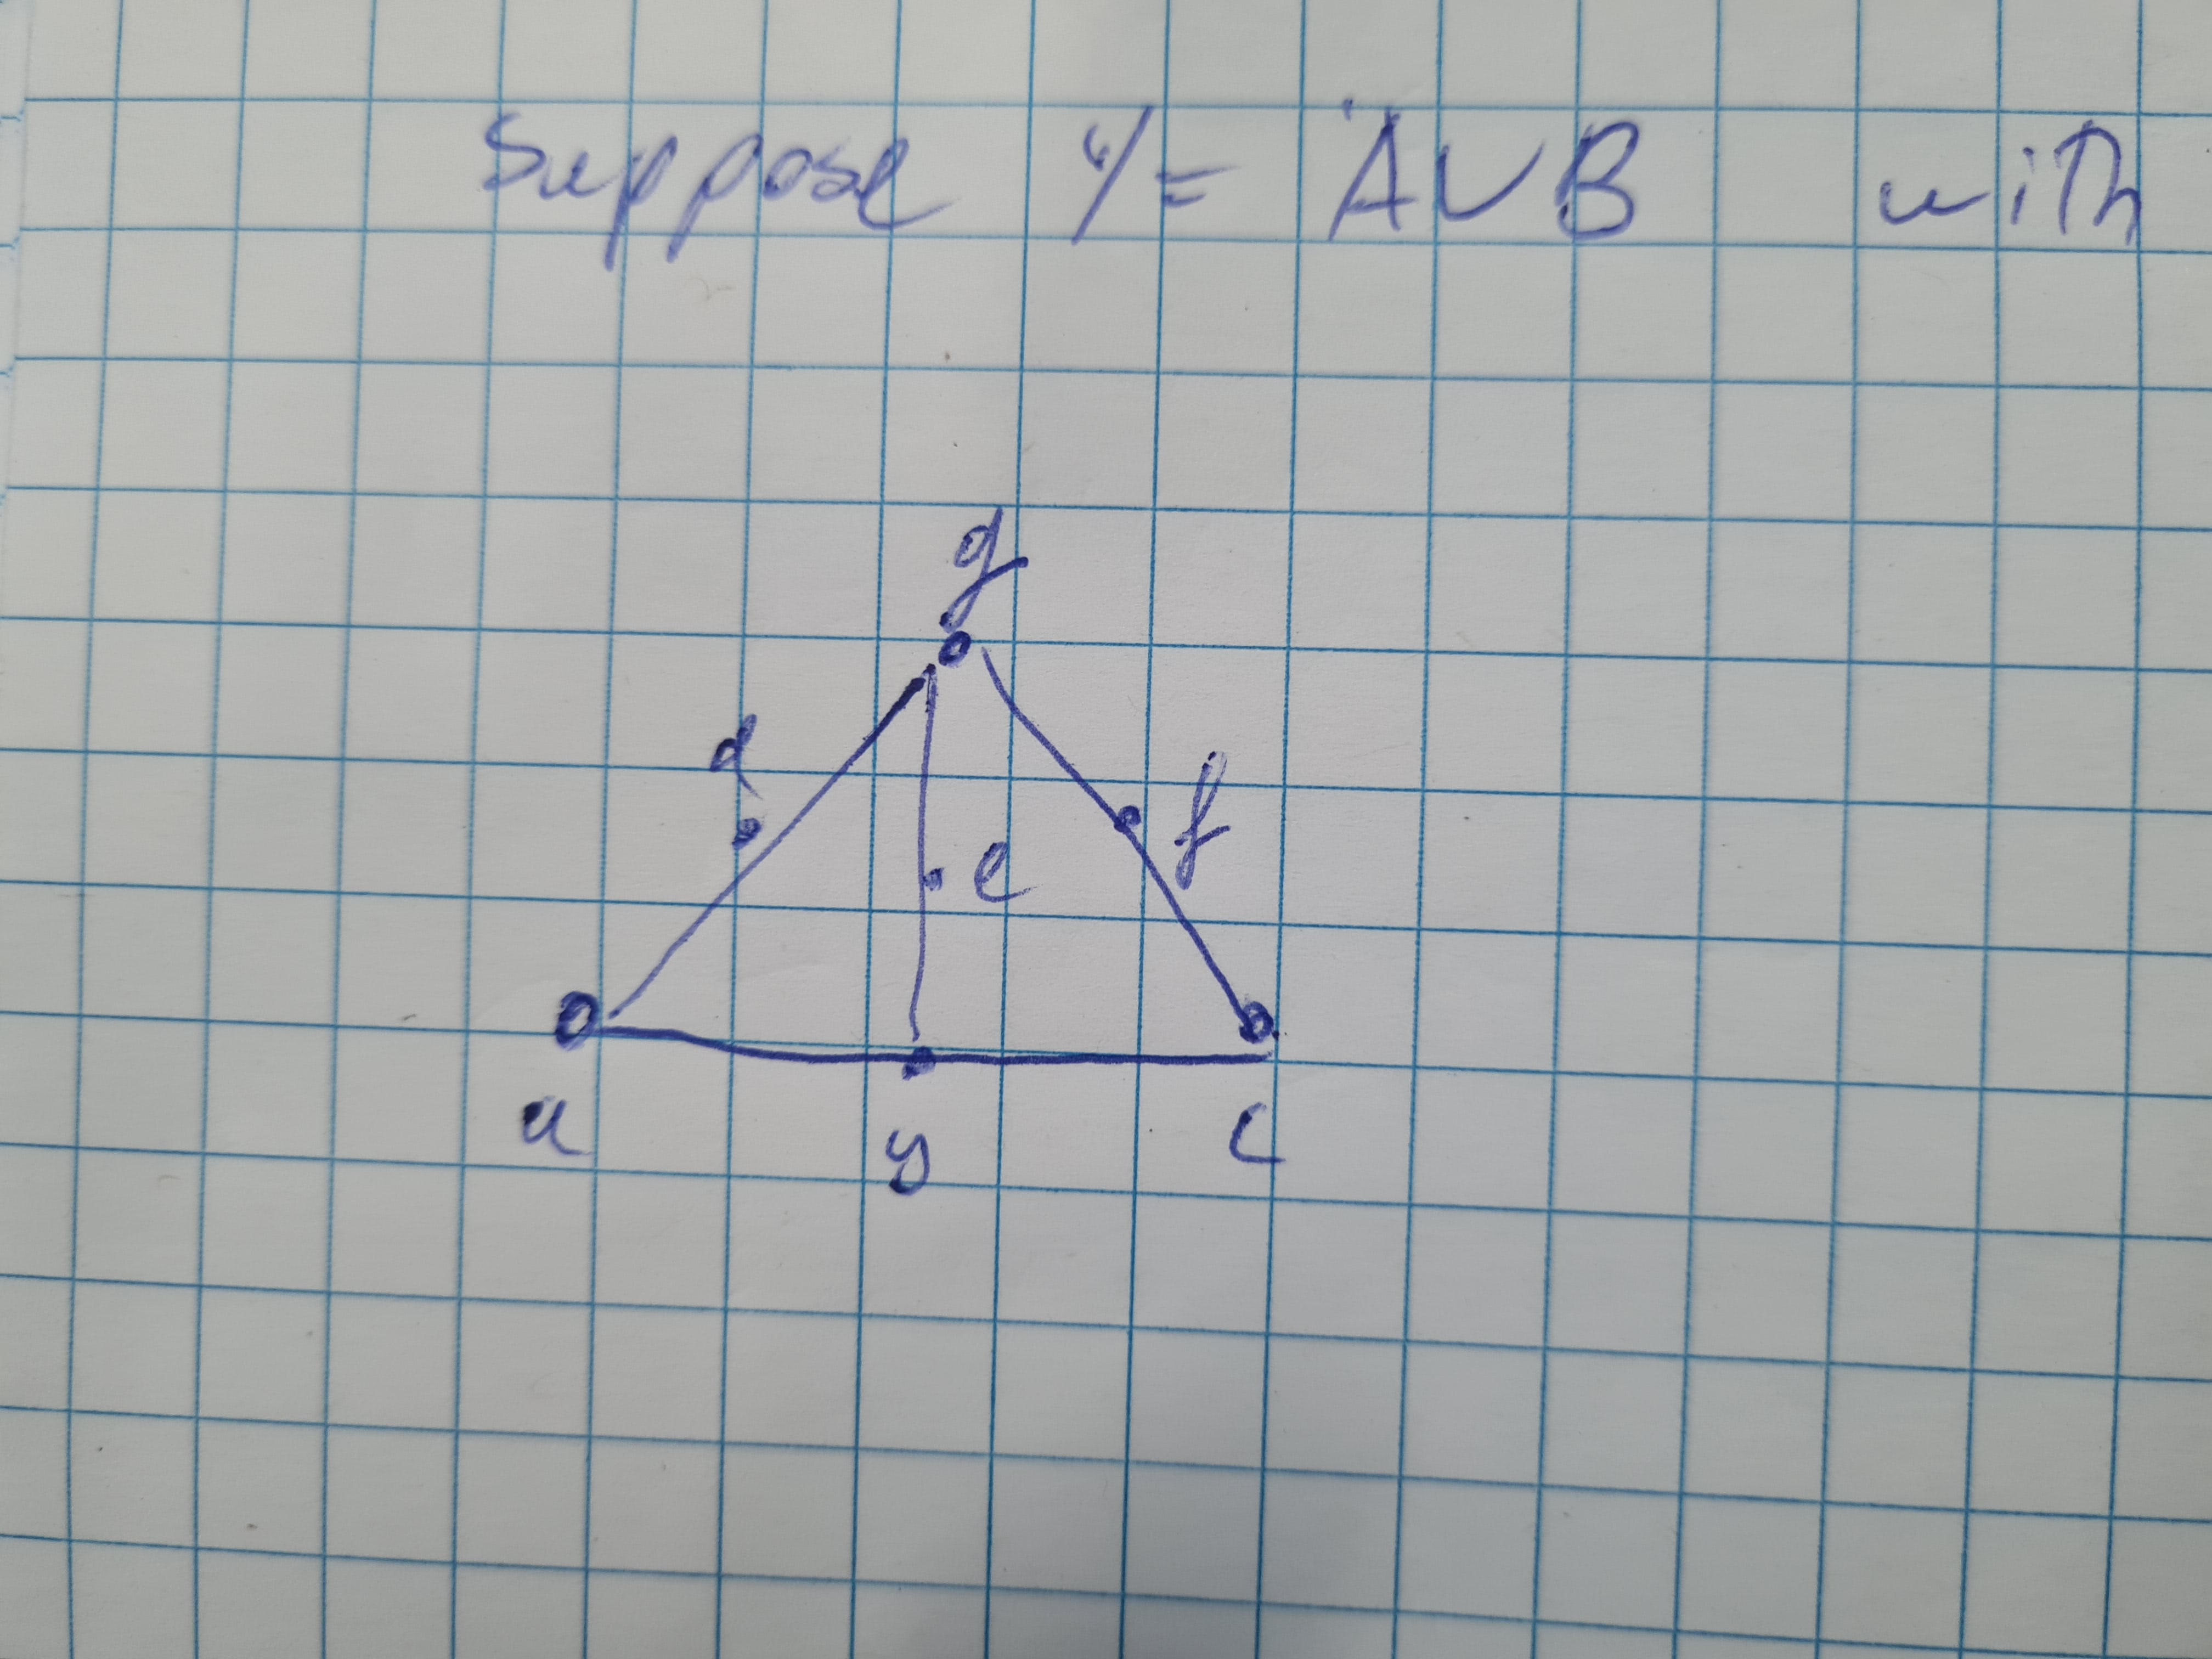
\includegraphics[width=0.5\textwidth]{q6a.jpg}
            \caption{geometric representation of $M$}
        \end{figure}

\begin{figure}
    \centering
            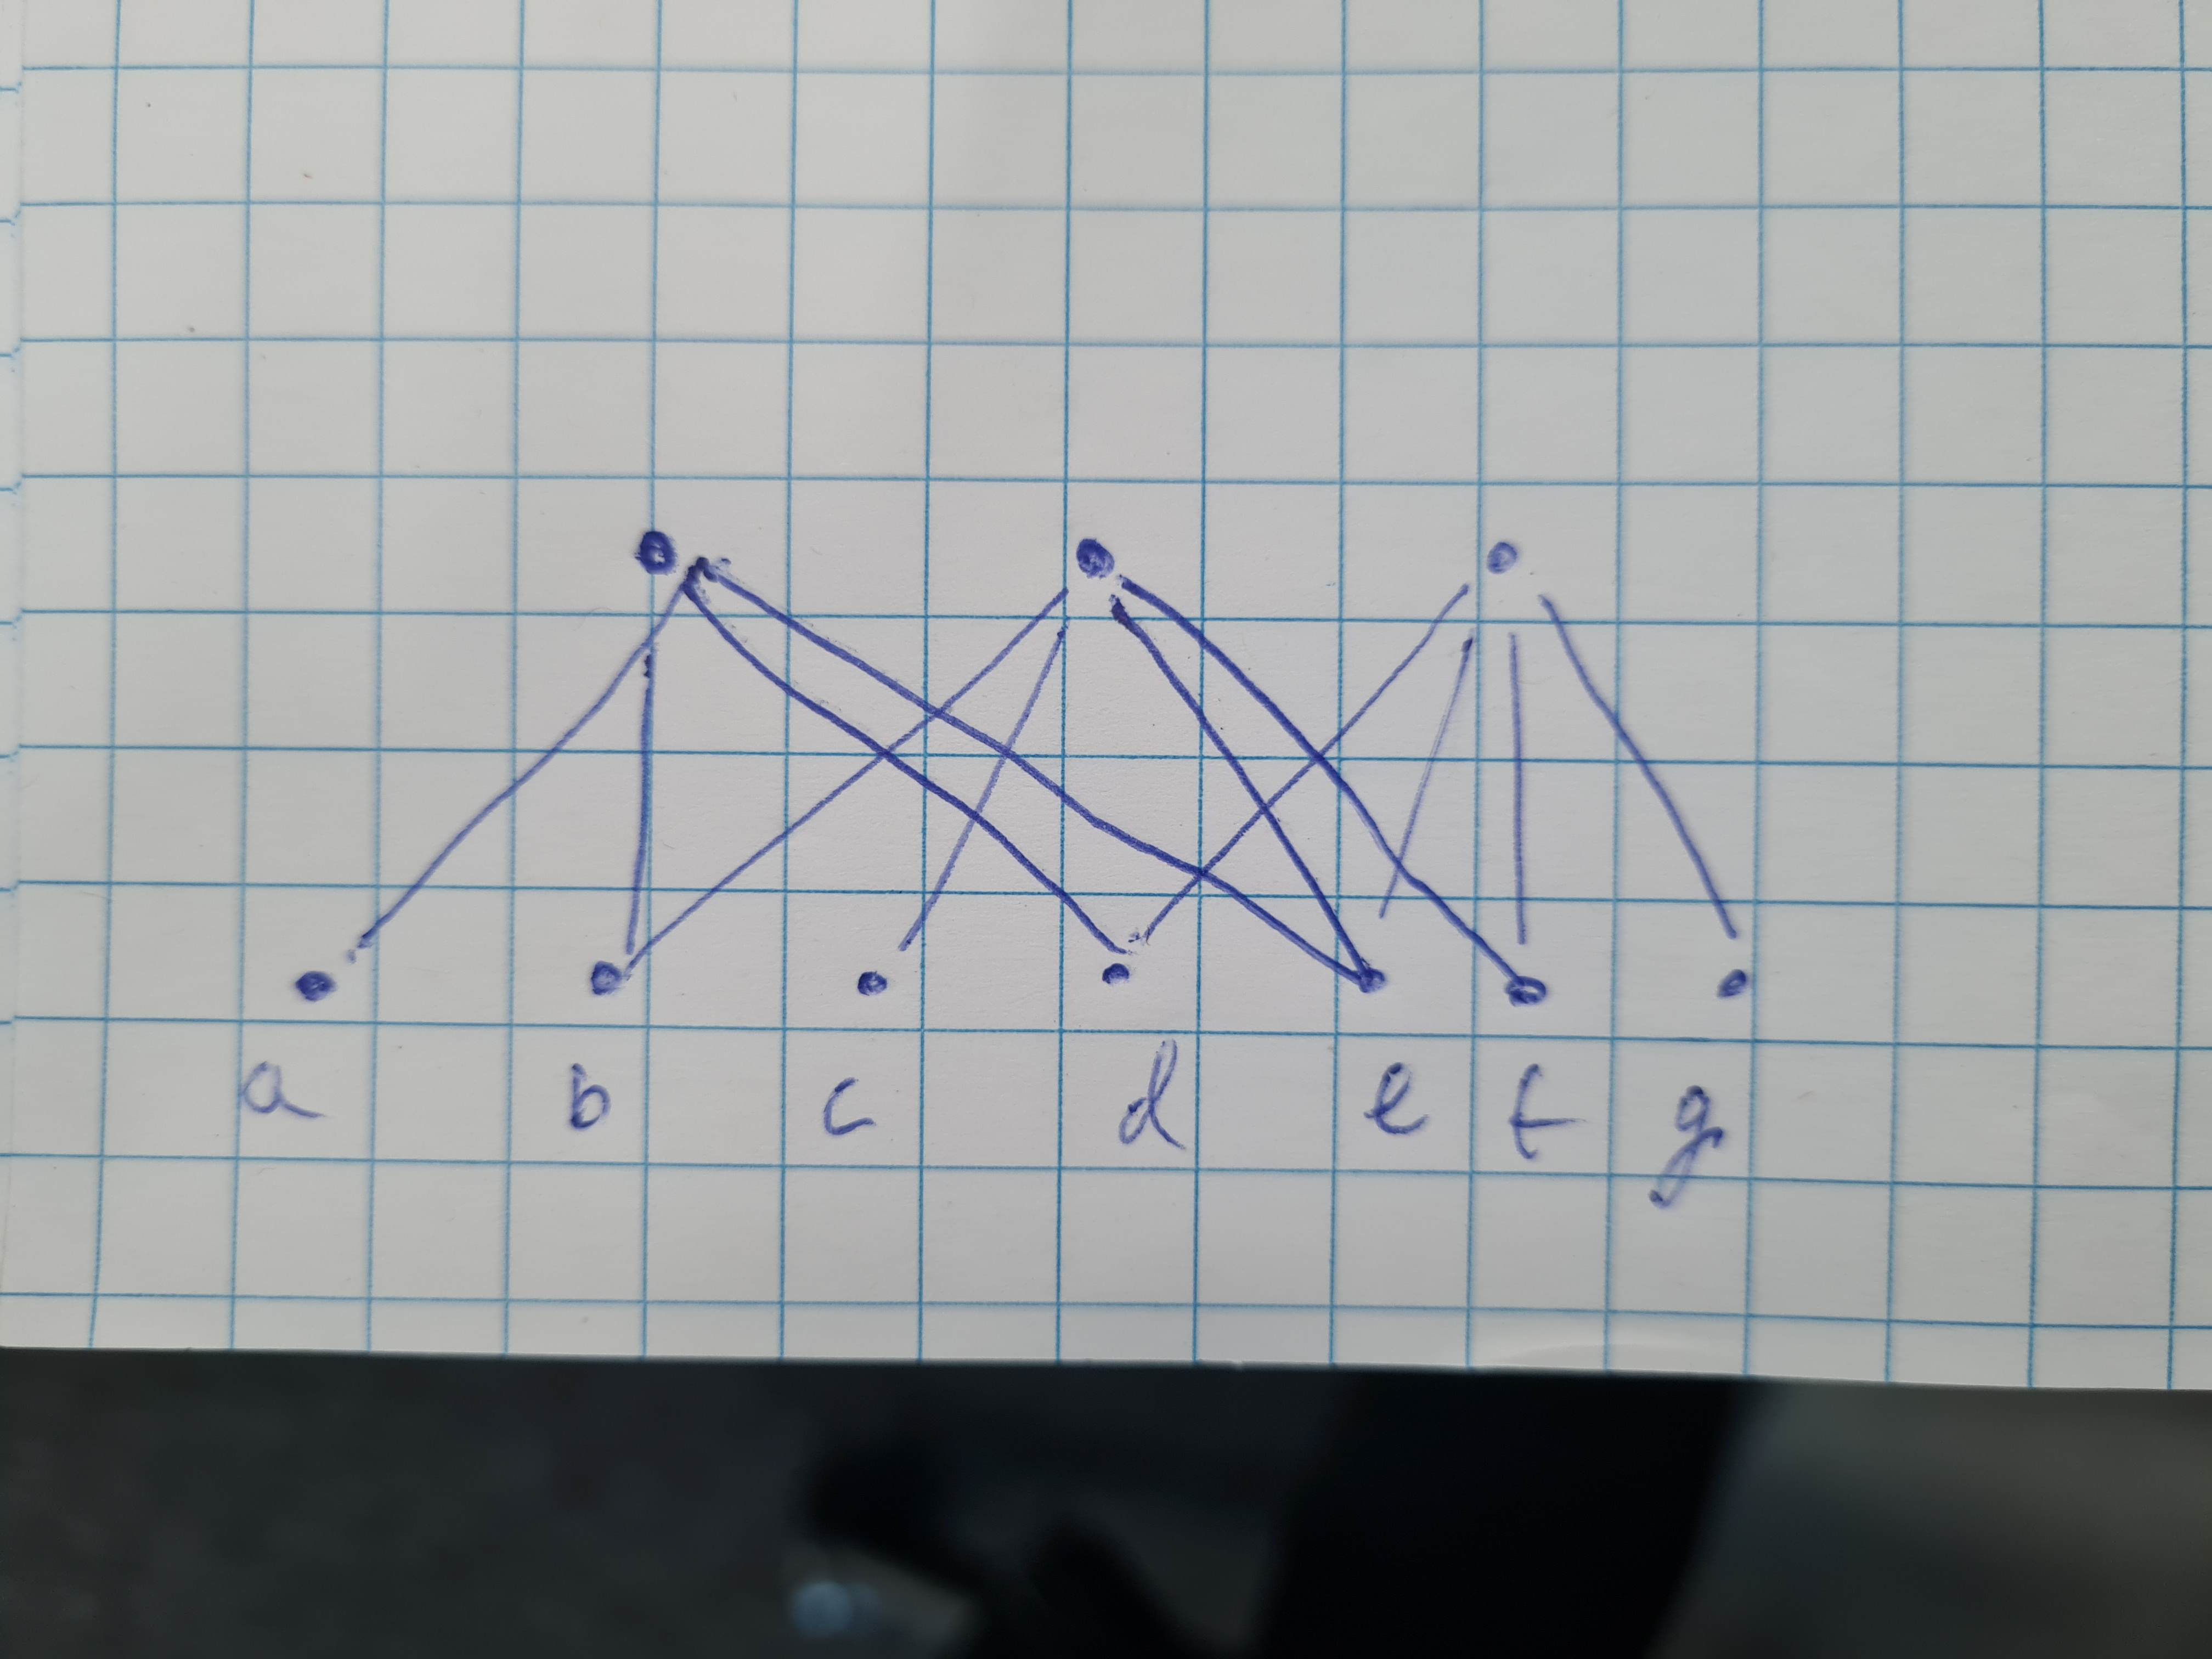
\includegraphics[width=0.5\textwidth]{q6b.jpg}
            \caption{transversal representation of $M$}
        \end{figure}
When we contract along g, we obtain the following matroid, $M/e$, seen in the figure.
\begin{figure}
    \centering
            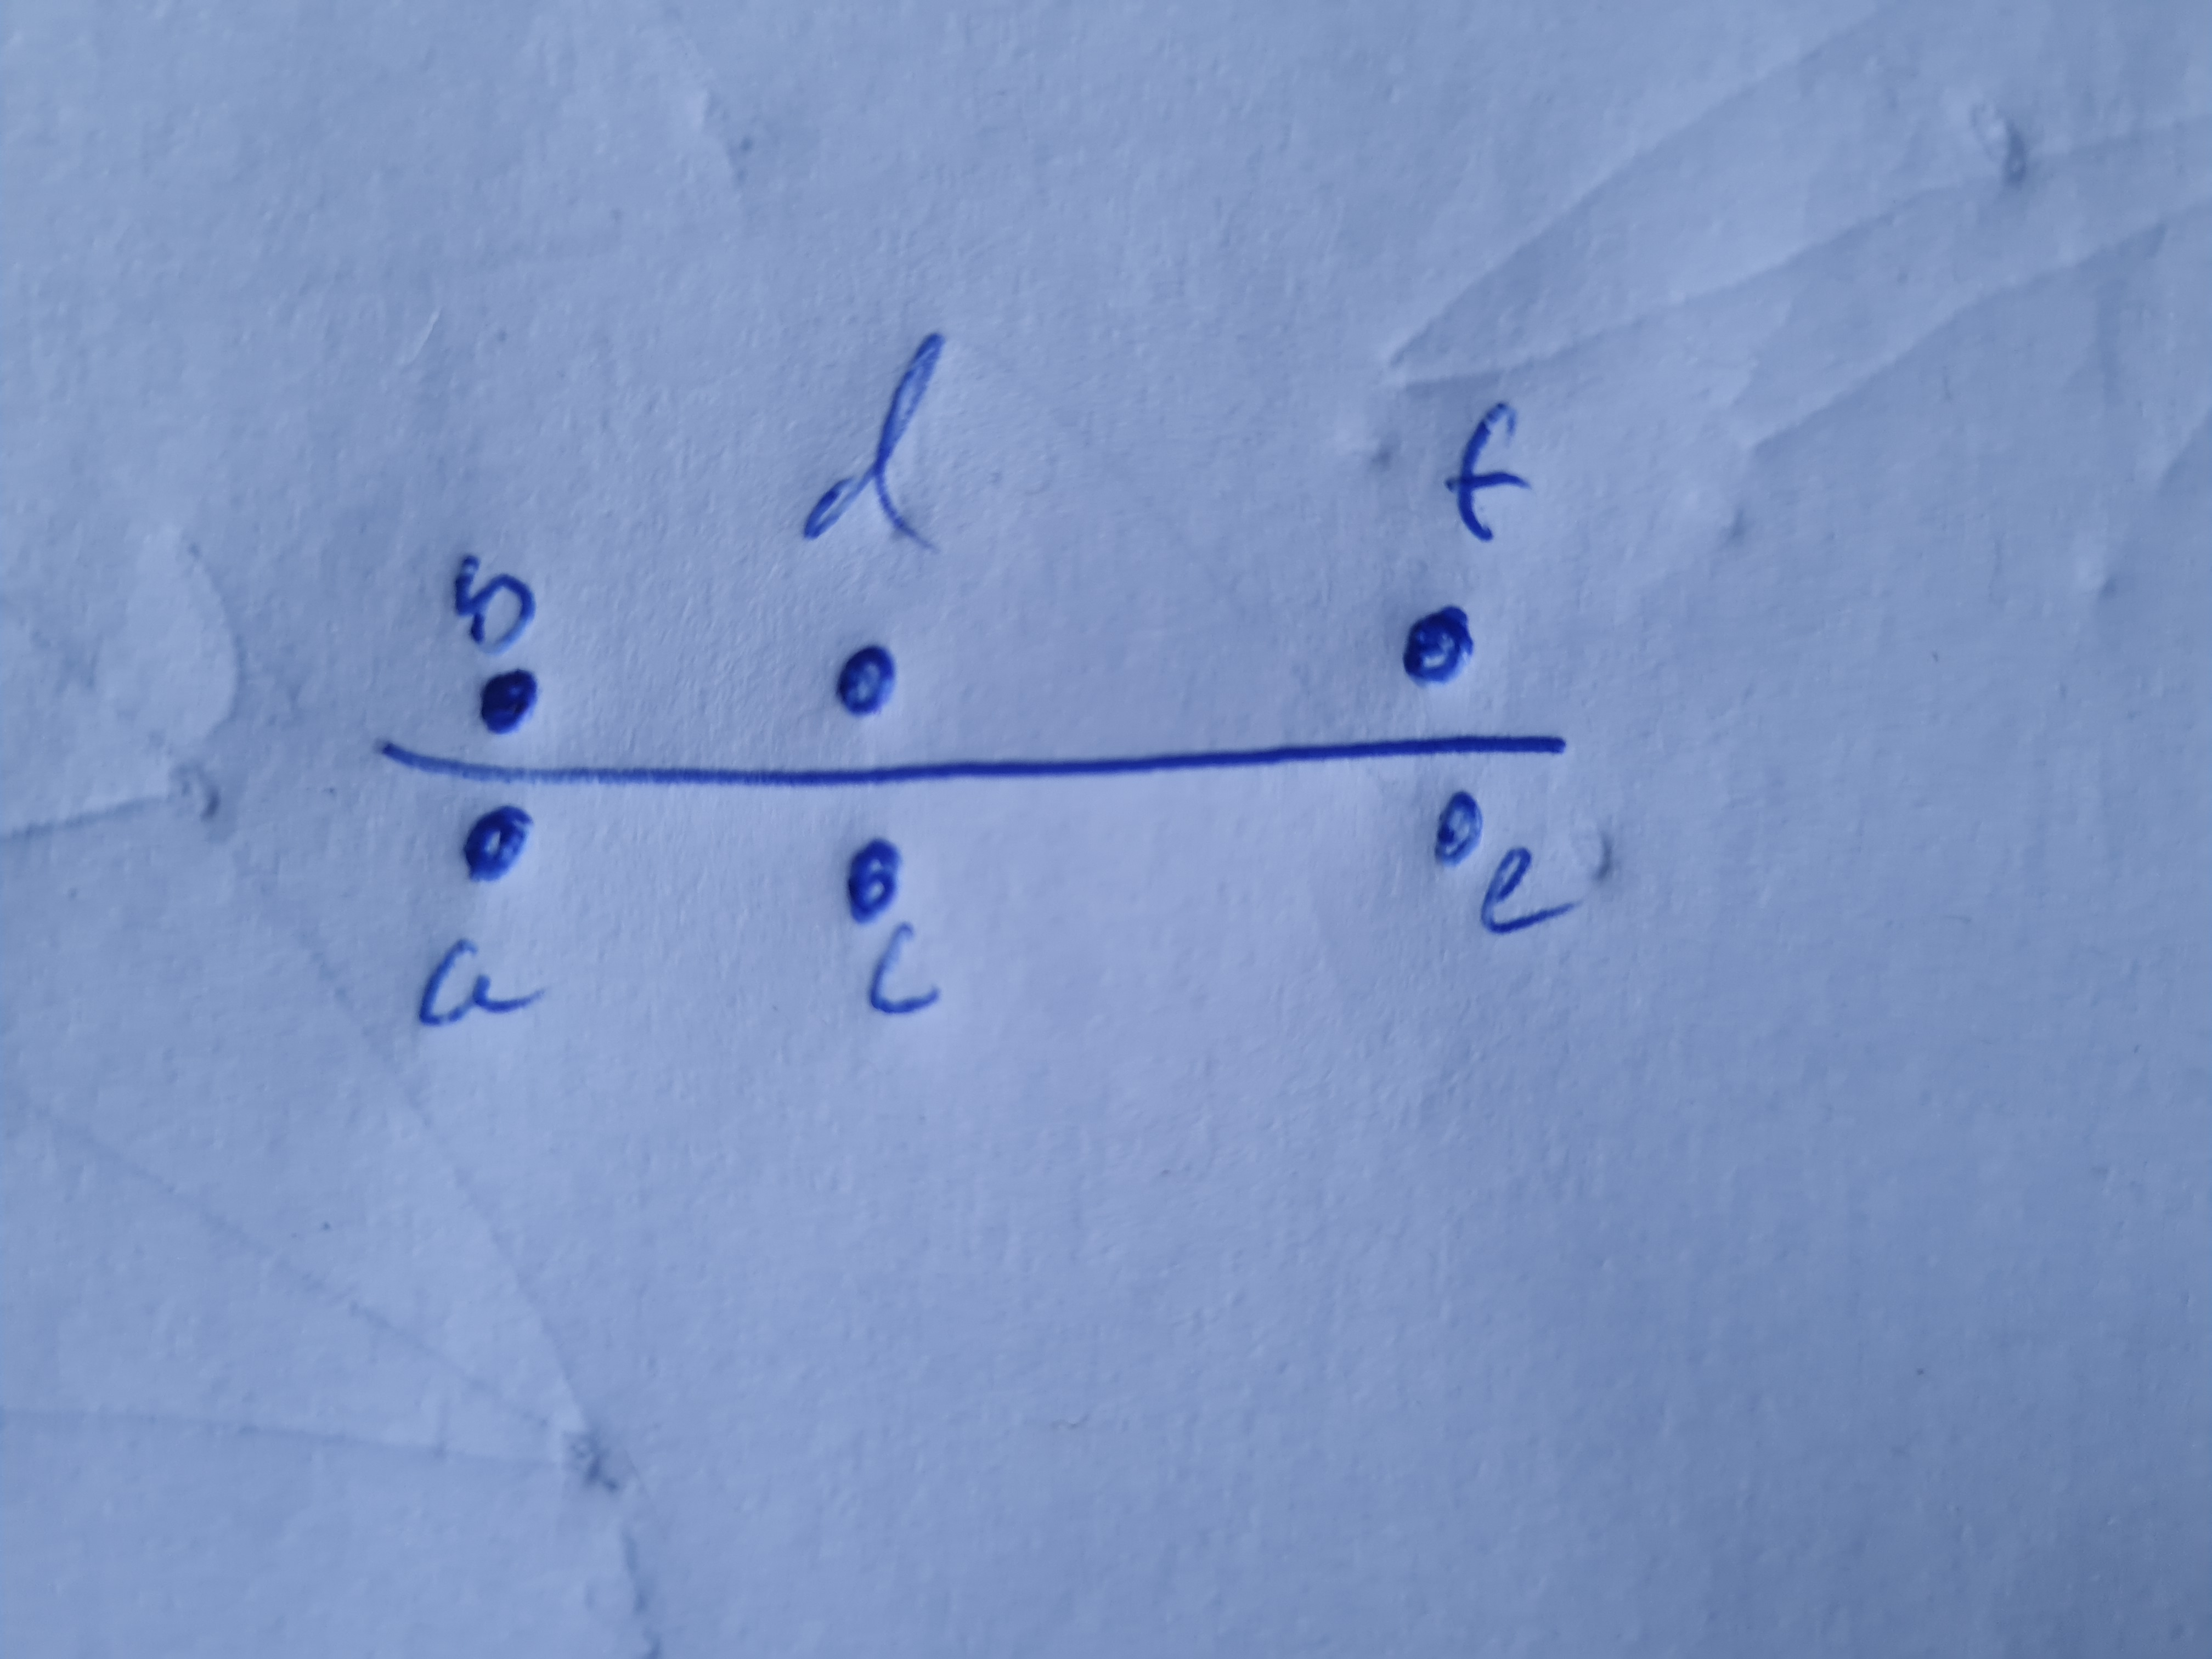
\includegraphics[width=0.5\textwidth]{q6main.jpg}
            \caption{geometric representation of $M/e$, which we know is not transversal.}
        \end{figure}
This is exactly the same matroid that I showed was not transversal in the previous assignment 
(I got full marks in that question so I hope I can just refer you to that assignment for an argument?)

\end{document}